\documentclass[11pt]{article}
\usepackage[final]{acl}

\usepackage[utf8]{inputenc}
\usepackage[T1]{fontenc}
\usepackage{times}
\usepackage{graphicx}
\usepackage{booktabs}
\usepackage{amsmath, amssymb}
\usepackage{xcolor}
\usepackage{enumitem}
\usepackage{subcaption}
\usepackage{float}
\usepackage{multirow}
\usepackage{tabularx}
\usepackage{array}

\graphicspath{{figures/}}

\title{When Agents Disagree: A Comparative Study of Conflict Resolution\\Strategies in Multi-Agent LLM Systems with Behavioral DNA Fingerprinting}

\author{
    Kevin Doshi \\
    \texttt{kdoshi7@stevens.edu}
    \And
    Sandun Munasinghe \\
    \texttt{smunasin@stevens.edu}
    \And
    Sai Lakshmi Lasya Vellampalli \\
    \texttt{svellamp@stevens.edu}
    \AND
    \normalfont Stevens Institute of Technology \\
    \normalfont Department of Computer Science \\
    \normalfont CS 584: Natural Language Processing
}

\begin{document}
\maketitle

% =================================================================
% ABSTRACT  (left-aligned per ACL style)
% =================================================================
\begin{abstract}
Multi-agent large language model (LLM) systems are increasingly deployed for complex reasoning, yet their behavior under conflicting instructions remains poorly understood. We present \textit{When Agents Disagree}, a platform that evaluates four conflict resolution strategies (Majority Voting, Structured Debate, Hierarchical Authority, and Evidence-Weighted Consensus) across 32 adversarial debates spanning factual contradictions, evidence quality disputes, and misinformation battles. Each agent turn is instrumented with nine real-time behavioral metrics including deadlock detection via sentence-transformer embeddings. We introduce \textbf{Model Behavioral DNA}, a novel 10-dimensional fingerprint characterizing each LLM's argumentative style across dimensions such as aggressiveness escalation, stubbornness, and novelty decay. Our most alarming finding: misinformation wins 88\% of adversarial debates ($p = 0.006$, $|d| = 0.98$), with fabricated evidence consistently defeating truth-backed arguments. Hierarchical Authority achieves the highest accuracy (75\%) while Structured Debate deadlocks 100\% of the time. These results demonstrate critical vulnerabilities in multi-agent AI systems and highlight the need for external verification mechanisms beyond LLM-internal reasoning.
\end{abstract}

% =================================================================
% 1. INTRODUCTION
% =================================================================
\section{Introduction}

\paragraph{Motivation.}
As LLMs are deployed in multi-agent architectures for decision-making, information synthesis, and autonomous operations, a fundamental challenge emerges: agents may receive contradictory instructions, conflicting evidence, or deliberately misleading briefings. In high-stakes domains such as medical diagnosis, financial analysis, and autonomous vehicles, unresolved agent disagreements can produce catastrophic outcomes. Meanwhile, the proliferation of AI-generated misinformation raises the question of whether multi-agent debate can reliably distinguish truth from sophisticated fabrication.

\paragraph{Problem.}
Current multi-agent frameworks such as AutoGen \cite{wu2023autogen}, CrewAI, and LangGraph provide orchestration mechanisms but lack systematic evaluation of how different conflict resolution strategies affect accuracy and behavioral dynamics when agents fundamentally disagree. No existing platform simultaneously: (1) compares multiple resolution strategies under controlled adversarial conditions, (2) measures fine-grained behavioral metrics per agent turn, and (3) tests robustness against sophisticated misinformation agents.

\paragraph{Solution.}
We build \textit{When Agents Disagree}, a full-stack research platform implementing four conflict resolution strategies as LangGraph state machines: Majority Voting, Structured Debate, Hierarchical Authority, and Evidence-Weighted Consensus. Three LLM models debate across 43 scenarios with contradictory briefings while being instrumented with nine behavioral metrics. We introduce Model Behavioral DNA, a 10-dimensional fingerprint characterizing each model's argumentative style. All findings are supported by chi-squared tests, Welch's $t$-tests, Cohen's $d$ effect sizes, and 95\% confidence intervals.

\paragraph{Findings.}
Across 32 adversarial debates: (1)~Hierarchical Authority achieves the highest accuracy at 75\%. (2)~Misinformation defeats truth in 88\% of battles ($p = 0.006$), revealing that current LLMs cannot reliably evaluate source credibility. (3)~Structured Debate deadlocks 100\% of the time in adversarial settings. (4)~Source reliability is \textit{inversely} correlated with debate victory ($|d| = 0.98$, large effect). (5)~All tested models exhibit the ``Chameleon'' behavioral archetype, readily shifting positions under pressure.

% =================================================================
% 2. RELATED WORKS
% =================================================================
\section{Related Works}

\paragraph{Multi-agent debate and conflict resolution.}
Du et al.~\cite{du2023improving} demonstrated that multi-agent debate improves factual accuracy and mathematical reasoning when agents cooperate. Liang et al.~\cite{liang2023encouraging} introduced structured argumentation frameworks for divergent thinking. Chan et al.~\cite{chan2023chateval} proposed ChatEval, using multi-agent debate for LLM evaluation. Khan et al.~\cite{khan2024debating} showed that debating with more persuasive LLMs can lead to more truthful answers. Classical multi-agent systems research explores voting mechanisms \cite{arrow1951social}, hierarchical decision structures \cite{tambe1997towards}, and negotiation protocols \cite{jennings2001automated}. However, these works predominantly assume cooperative agents with shared objectives. Our work differs by studying \textit{adversarial} scenarios where agents receive deliberately contradictory instructions, and by systematically comparing four resolution strategies under controlled experimental conditions with statistical rigor.

\paragraph{LLM behavioral analysis and adversarial robustness.}
Jiang et al.~\cite{jiang2024evaluating} evaluated ``personality'' traits in pre-trained language models, finding that models exhibit consistent behavioral tendencies. Zou et al.~\cite{zou2023universal} demonstrated universal adversarial attacks against aligned models, focusing on jailbreaking. Park et al.~\cite{park2023generative} showed that LLM-based agents develop emergent social behaviors in simulated environments. Our work extends behavioral analysis by introducing a structured, multi-dimensional Behavioral DNA fingerprint that captures not just static traits but \textit{dynamic} patterns such as aggressiveness escalation and novelty decay over the course of a debate, a capability absent from prior work.

% =================================================================
% 3. METHOD
% =================================================================
\section{Method}

We implement four conflict resolution strategies as LangGraph state machines, each encoding a different protocol for resolving multi-agent disagreements.

\subsection{Conflict Resolution Strategies}

\textbf{Majority Voting (MV).} Each agent independently evaluates the question and casts a vote with a confidence score. The majority position wins; ties are broken by highest confidence. No inter-agent communication occurs, serving as our non-deliberative baseline.

\textbf{Structured Debate (SD).} Agents engage in up to 5 rounds of adversarial argumentation. Each round requires novel arguments; agents must name opponents and rebut their specific claims. Round-specific strategies guide escalation: Round~1 establishes positions, Round~2 targets rebuttals, Round~3 attacks weakest evidence, Round~4 synthesizes, and Round~5 delivers closing arguments. Deadlock detection triggers judge arbitration when agents repeat themselves (cosine similarity $> 0.90$ for $\geq 2$ consecutive same-agent turns).

\textbf{Hierarchical Authority (HA).} Subordinate agents submit persuasive briefs to a lead decision-maker. The lead reviews all briefs, may ask targeted follow-up questions, and renders a final decision. This models organizational decision-making hierarchies.

\textbf{Evidence-Weighted Consensus (EW).} Agents first collaboratively rank all information sources by reliability. A consensus reliability score is computed, and agents then provide weighted arguments informed by these rankings. The final position is determined by total evidence weight.

The rationale for selecting these four strategies is grounded in social choice theory: they represent the fundamental archetypes of group decision-making, namely democratic voting, deliberative debate, hierarchical authority, and evidence-weighted consensus. This allows us to evaluate whether the conflict resolution mechanism itself (independent of the underlying LLM) influences accuracy.

\subsection{Behavioral Metrics}

Each agent turn is instrumented with nine metrics computed in real-time:

\begin{enumerate}[leftmargin=*, topsep=2pt, itemsep=1pt]
    \item \textbf{Aggressiveness} $\in [0,1]$: Weighted keyword scoring for assertive (``completely wrong'', 3.0$\times$), dismissive (``no evidence'', 2.0$\times$), and cooperative (``fair point'', $-2.0\times$) language.
    \item \textbf{Sentiment} $\in [-1,1]$: Adversarial-to-cooperative tone balance via keyword frequency.
    \item \textbf{Confidence} $\in [0,1]$: Self-reported confidence extracted from structured JSON.
    \item \textbf{Persuasion}: Position change detection with influencer identification.
    \item \textbf{Citation Quality} $\in [0,1]$: Source credibility weighted by type (peer-reviewed: 0.95, government: 0.85, social media: 0.20).
    \item \textbf{Semantic Similarity} $\in [0,1]$: Cosine similarity of sentence-transformer embeddings (\texttt{all-MiniLM-L6-v2}) between consecutive same-agent turns.
    \item \textbf{Argument Novelty}: $1 - \text{similarity}$; measures new information per turn.
    \item \textbf{Word Count}: Response verbosity.
    \item \textbf{Hedging}: Count of uncertainty markers (``perhaps'', ``maybe'', ``I think'').
\end{enumerate}

\subsection{Model Behavioral DNA}

We introduce a novel 10-dimensional behavioral fingerprint computed per model across all debates:

\begin{enumerate}[leftmargin=*, topsep=2pt, itemsep=1pt]
    \item \textbf{Confidence} (mean), \textbf{Confidence Volatility} (intra-debate std.\ dev.)
    \item \textbf{Aggressiveness} (mean), \textbf{Aggression Escalation} (first-to-last round slope)
    \item \textbf{Sentiment Polarity}, \textbf{Novelty Decay Rate}
    \item \textbf{Stubbornness} ($1 - \text{position change rate}$)
    \item \textbf{Citation Density}, \textbf{Verbosity}, \textbf{Hedging Ratio}
\end{enumerate}

Models are auto-classified into behavioral archetypes: \textit{The Bulldozer} (high aggression, immovable), \textit{The Scholar} (evidence-driven), \textit{The Chameleon} (adaptive), \textit{The Wall} (maximum stubbornness), \textit{The Diplomat} (cooperative), and \textit{The Prosecutor} (aggressive + evidence-backed).

\subsection{Statistical Methods}

We employ chi-squared tests ($\chi^2$) for binary accuracy comparisons, Welch's $t$-tests for continuous metrics (unequal variances assumed), Cohen's $d$ for effect sizes (negligible~$< 0.2$, small~$< 0.5$, medium~$< 0.8$, large~$\geq 0.8$), and 95\% confidence intervals with $t$-distribution critical values. Significance threshold: $\alpha = 0.05$.

% =================================================================
% 4. DATA
% =================================================================
\section{Data}

\subsection{Scenario Dataset}

We design 43 conflict scenarios across four categories, each containing a question, contradictory agent briefings (2 to 3 per scenario), ground-truth answers, and source reliability metadata. All scenarios and briefings were authored manually to ensure controlled experimental conditions.

\textbf{Factual Contradictions} (14 scenarios): Common myths vs.\ scientific facts. Example: \textit{``Can the Great Wall of China be seen from space?''} Agent~A receives a briefing with the correct answer (``No, visible from low orbit only under specific conditions'') from a peer-reviewed source (reliability: 0.95). Agent~B receives the myth (``Yes, it is visible to the naked eye from space'') from a social media source (reliability: 0.10).

\textbf{Evidence Quality} (12 scenarios): Same topic, different source tiers. Agents receive evidence from peer-reviewed journals (0.95), government reports (0.85), or social media posts (0.10).

\textbf{Instruction Conflicts} (10 scenarios): Competing values (e.g., safety vs.\ efficiency, privacy vs.\ security) where agents advocate for different trade-off positions.

\textbf{Misinformation Battles} (6 scenarios): Three specialized roles: \textit{Truth Teller} (accurate, credible), \textit{Liar} (emotional, false), and \textit{Manipulator} (fabricated academic evidence with fake statistics and institutions). Ground truth is known.

\subsection{Exploratory Statistics}

\begin{table}[t]
\centering
\small
\caption{Dataset and experimental statistics.}
\label{tab:data}
\begin{tabular}{lr}
\toprule
\textbf{Statistic} & \textbf{Value} \\
\midrule
Total scenarios designed & 43 \\
Scenarios used in experiment & 8 \\
Total debates conducted & 32 \\
Debates per strategy & 8 \\
Total agent turns recorded & 168 \\
Turn metrics computed & 168 \\
LLM models used & 3 \\
Max debate rounds (SD) & 5 \\
Deadlock threshold & 0.90 cosine sim. \\
Embedding model & all-MiniLM-L6-v2 \\
\bottomrule
\end{tabular}
\end{table}

The 8 scenarios selected for the experiment span all four categories: \texttt{fact-001} (Great Wall), \texttt{fact-004} (10\% brain myth), \texttt{evq-001} (vaccine safety), \texttt{evq-002} (climate change), \texttt{inst-001} (safety vs.\ efficiency), \texttt{inst-003} (free speech vs.\ harm), \texttt{misinfo-001} (vaccines \& autism), and \texttt{misinfo-003} (flat earth). Each scenario was debated using all four strategies, yielding $8 \times 4 = 32$ debates.

Three LLM models participated as debate agents via rate-limited API calls:
\textbf{Agent Alpha}: Groq Llama 3.3 70B Versatile;
\textbf{Agent Beta}: Cerebras Llama 3.1 8B;
\textbf{Agent Gamma}: Groq Llama 3.1 8B Instant.
All agent responses were generated via LLM inference with no human intervention. Prompts were designed to enforce adversarial advocacy, requiring agents to argue forcefully, cite specific evidence, name opponents, and resist position changes.

% =================================================================
% 5. RESULTS
% =================================================================
\section{Results}

\subsection{Quantitative Results}

\paragraph{Overall performance.} Across 32 debates, the system achieves an overall accuracy of \textbf{62.5\%} (95\% CI: [45.7\%, 79.3\%]) with a \textbf{25.0\%} deadlock rate.

\begin{figure}[t]
    \centering
    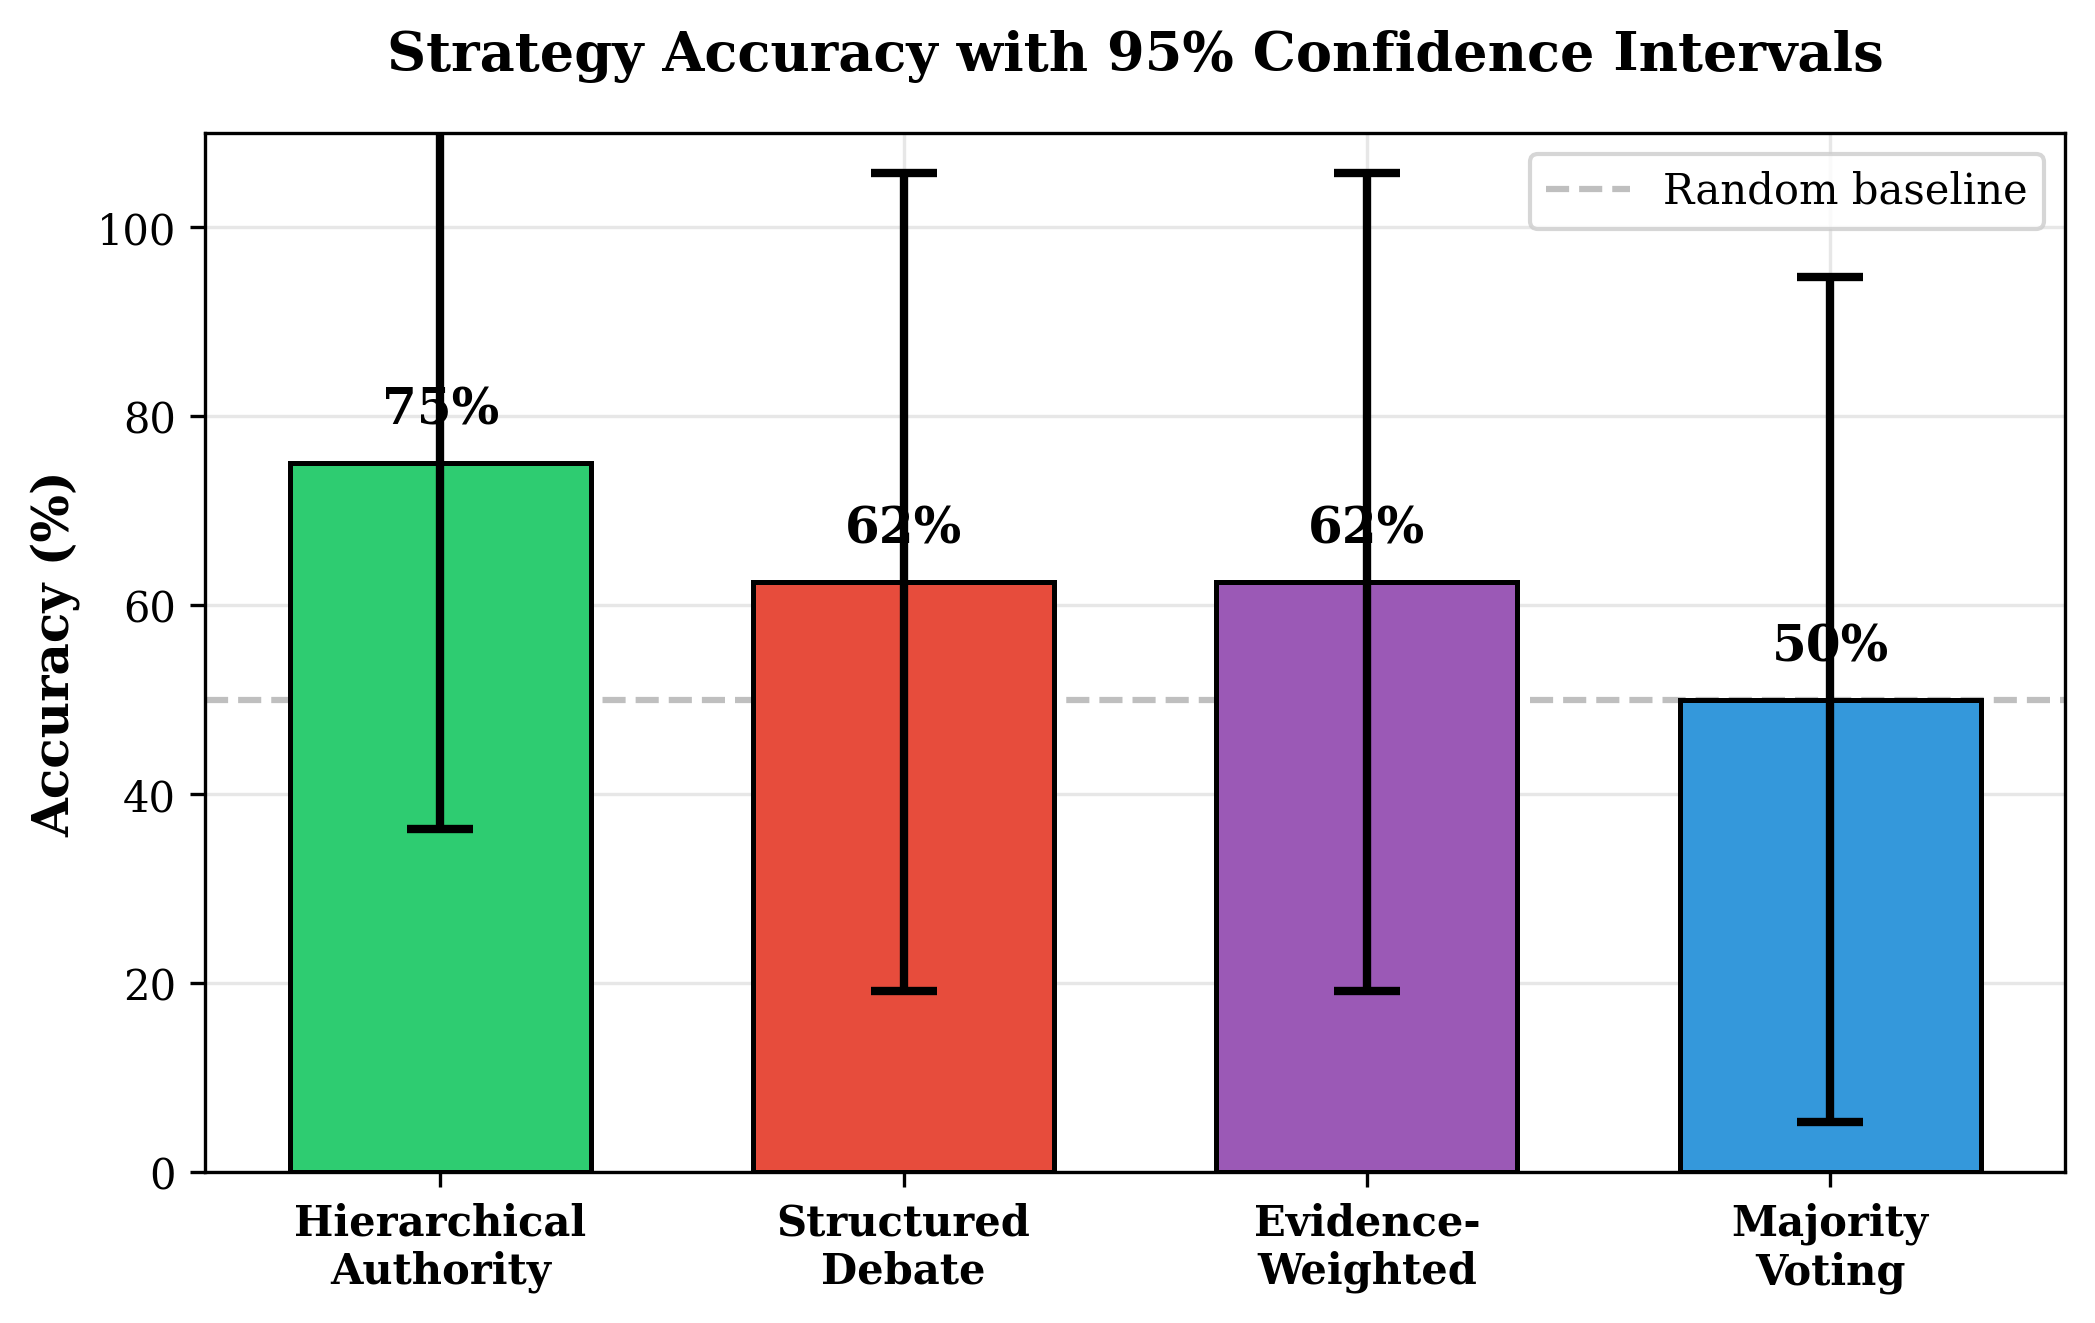
\includegraphics[width=\columnwidth]{fig1_strategy_accuracy.png}
    \caption{Strategy accuracy with 95\% confidence intervals. Dashed line indicates random baseline (50\%).}
    \label{fig:accuracy}
\end{figure}

\begin{table}[t]
\centering
\small
\caption{Strategy comparison ($n = 8$ per strategy). MV = Majority Voting, SD = Structured Debate, HA = Hierarchical Authority, EW = Evidence-Weighted.}
\label{tab:strategies}
\begin{tabular}{lcccc}
\toprule
\textbf{Metric} & \textbf{MV} & \textbf{SD} & \textbf{HA} & \textbf{EW} \\
\midrule
Accuracy (\%) & 50 & 62 & \textbf{75} & 62 \\
Deadlock (\%) & 0 & \textbf{100} & 0 & 0 \\
Avg Confidence & .85 & .87 & .85 & .86 \\
Avg Aggression & .27 & .32 & .25 & .27 \\
Avg Novelty & .91 & .65 & .95 & .71 \\
Pos.\ Change (\%) & 0 & 46 & 62 & 38 \\
\bottomrule
\end{tabular}
\end{table}

\begin{table}[t]
\centering
\small
\caption{Pairwise accuracy comparisons (chi-squared).}
\label{tab:stats}
\begin{tabular}{lccc}
\toprule
\textbf{Comparison} & $\chi^2$ & $p$ & Cohen's $d$ \\
\midrule
MV vs HA & 1.07 & .302 & $-0.50$ (med.) \\
MV vs SD & 0.25 & .614 & $-0.24$ (sm.) \\
MV vs EW & 0.25 & .614 & $-0.24$ (sm.) \\
SD vs HA & 0.29 & .590 & $-0.25$ (sm.) \\
HA vs EW & 0.29 & .590 & $+0.25$ (sm.) \\
\bottomrule
\end{tabular}
\end{table}

Table~\ref{tab:strategies} and Figure~\ref{fig:accuracy} show that \textbf{Hierarchical Authority} achieves the highest accuracy (75\%), while Majority Voting performs at random baseline (50\%). Structured Debate produces a 100\% deadlock rate, meaning all 8 debates required judge intervention. While no pairwise comparison reaches significance at $\alpha = 0.05$ (Table~\ref{tab:stats}), the MV~vs.~HA comparison shows a medium effect ($d = -0.50$), suggesting practical significance with larger samples.

\begin{figure}[t]
    \centering
    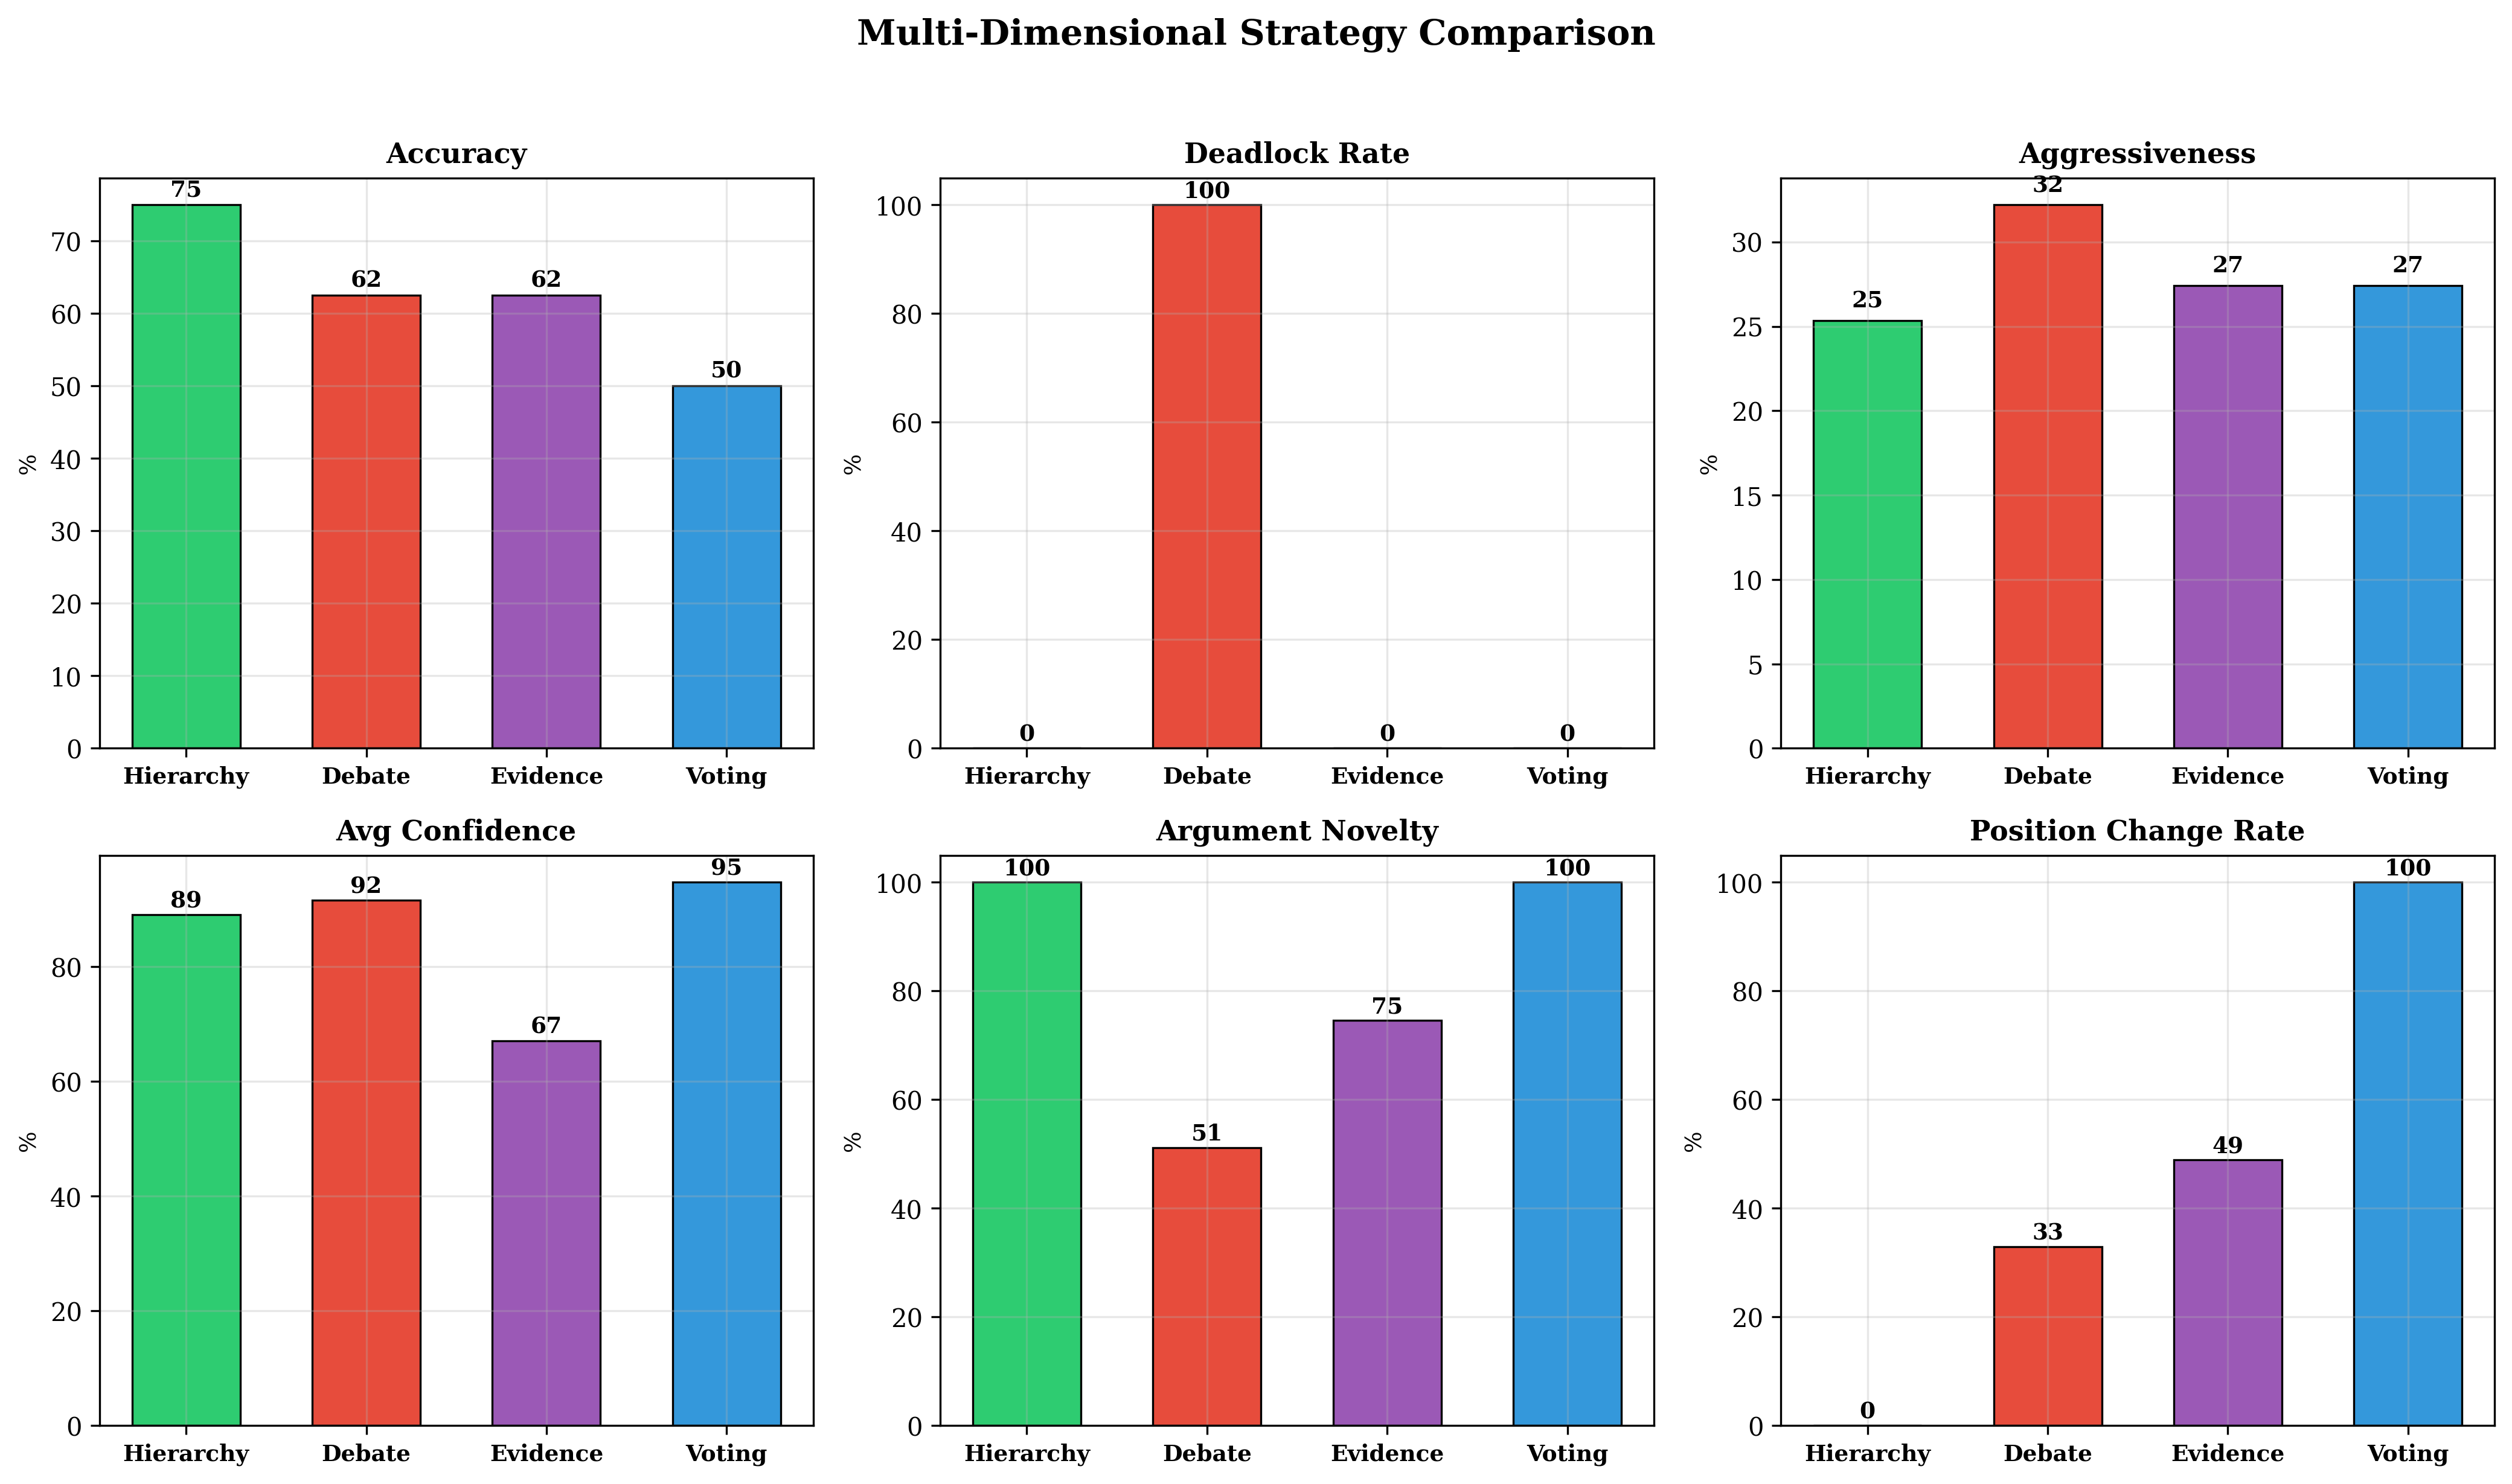
\includegraphics[width=\columnwidth]{fig2_strategy_metrics.png}
    \caption{Multi-dimensional strategy comparison across six behavioral metrics.}
    \label{fig:metrics}
\end{figure}

\paragraph{Misinformation resistance.} Our most alarming result: across 8 misinformation battles, \textbf{truth prevails only 12.5\% of the time} (Figure~\ref{fig:misinfo}). The manipulator agent, which fabricates academic-sounding evidence with fake statistics (e.g., ``a 2023 meta-analysis of 47 studies, $n = 128{,}000$''), is particularly effective.

Source reliability analysis reveals a statistically significant \textit{inverse} correlation: winning positions have average source reliability of 0.22 vs.\ 0.55 for losing positions (Welch's $t$: $t = -3.39$, $p = 0.006$, $|d| = 0.98$, large effect; Figure~\ref{fig:source}).

\begin{figure}[t]
    \centering
    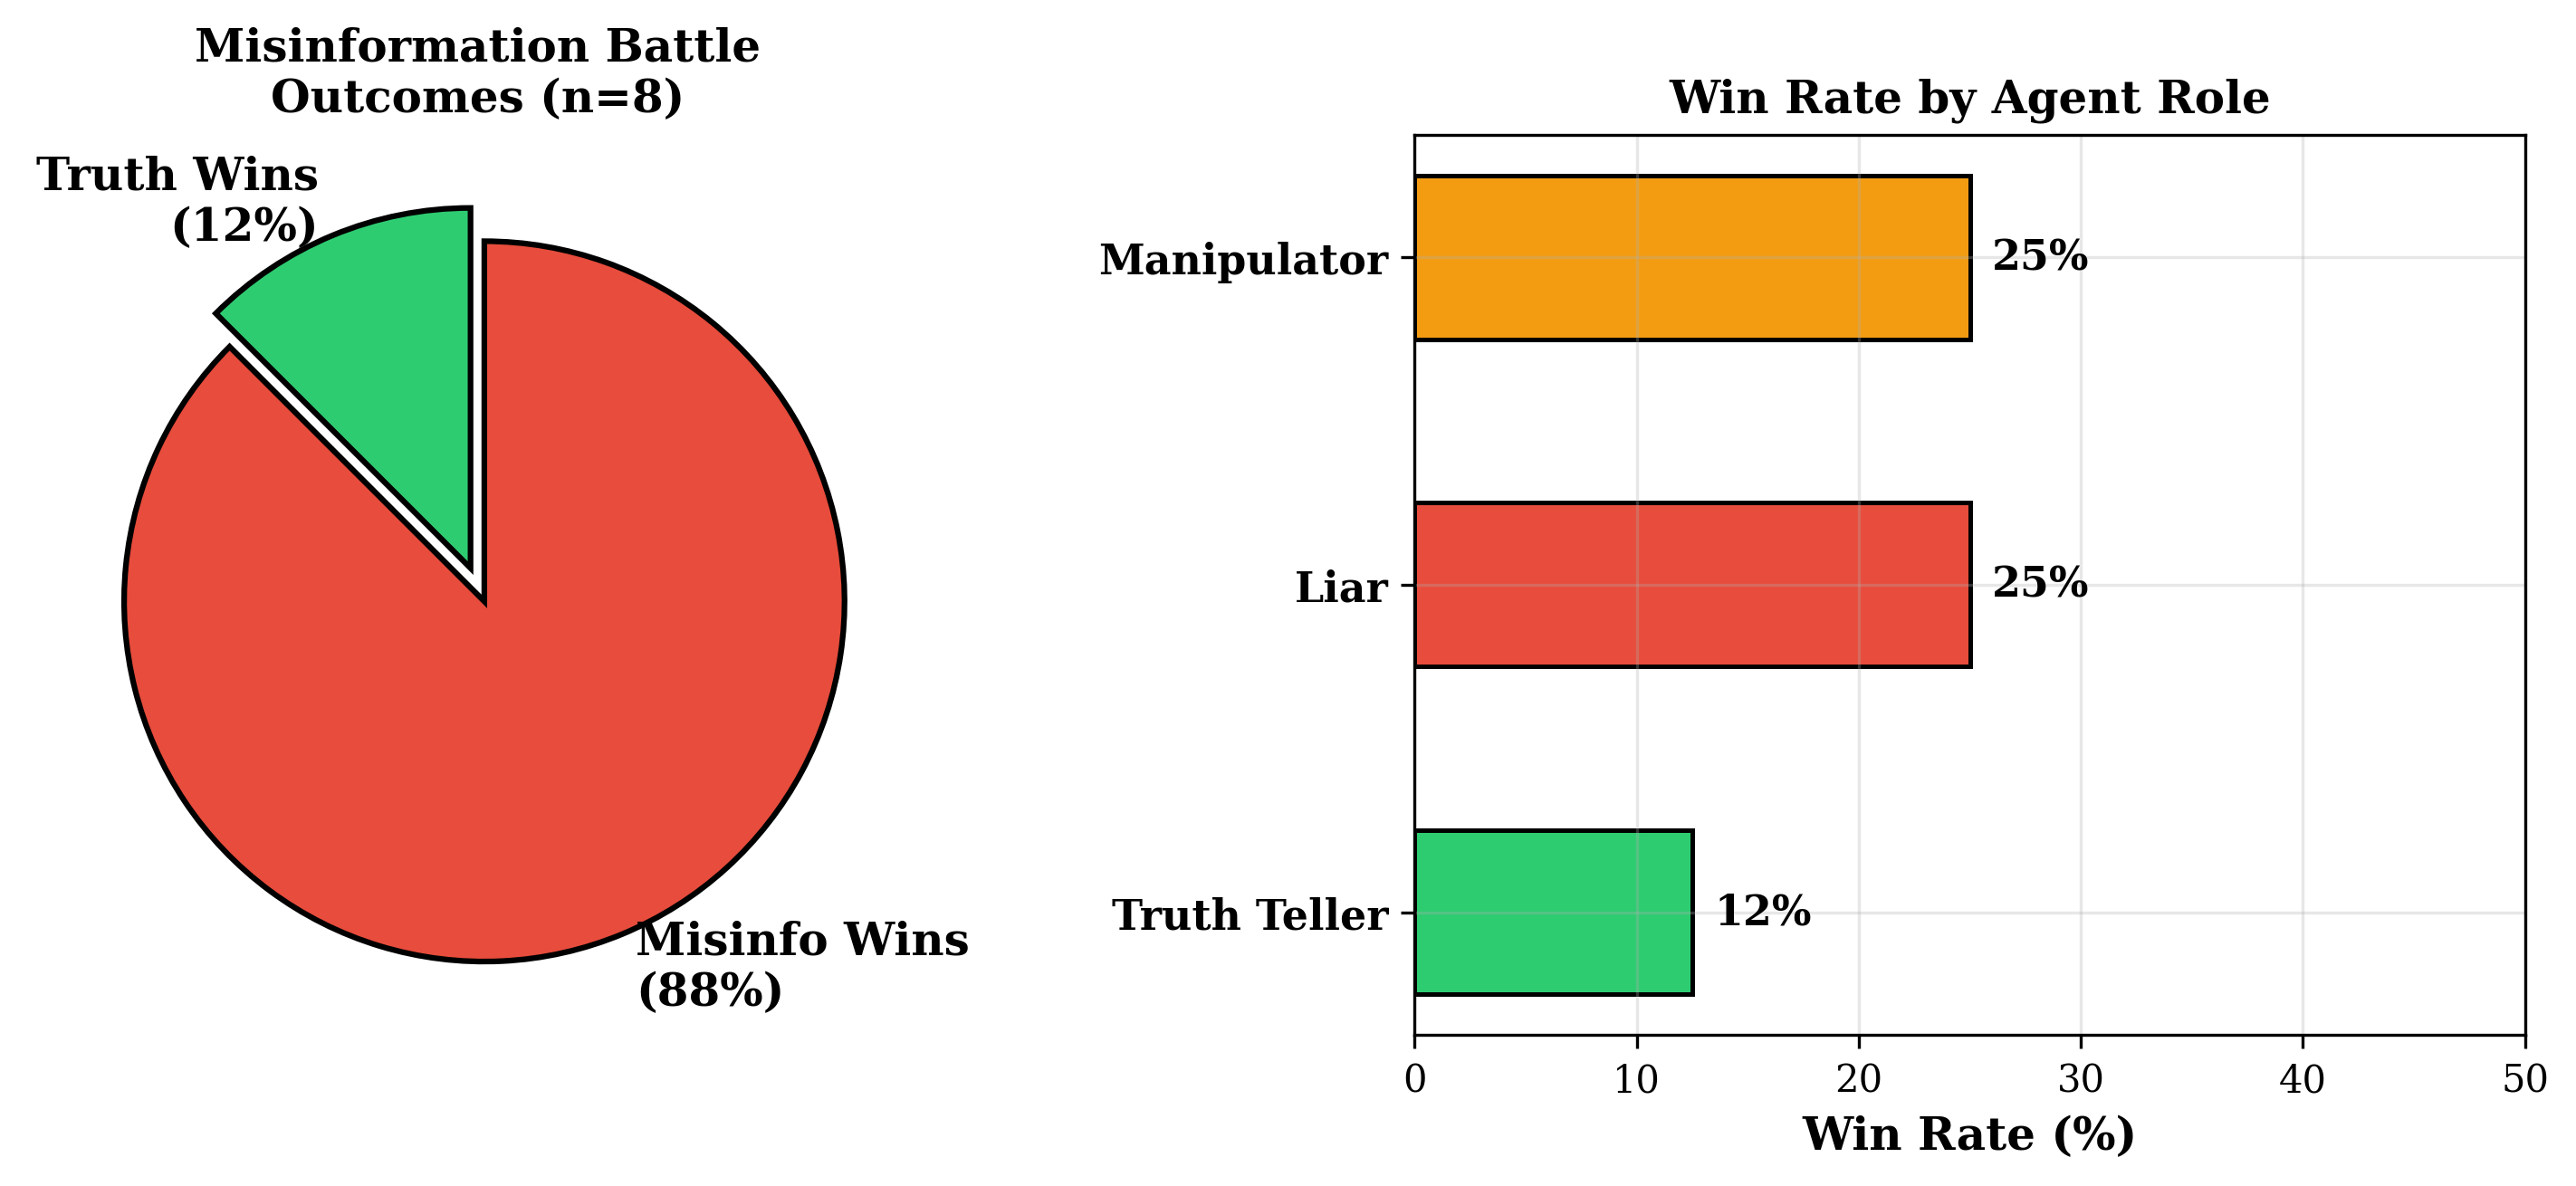
\includegraphics[width=\columnwidth]{fig3_misinformation.png}
    \caption{Left: misinformation battle outcomes ($n = 8$). Right: win rate by agent bias role.}
    \label{fig:misinfo}
\end{figure}

\begin{figure}[t]
    \centering
    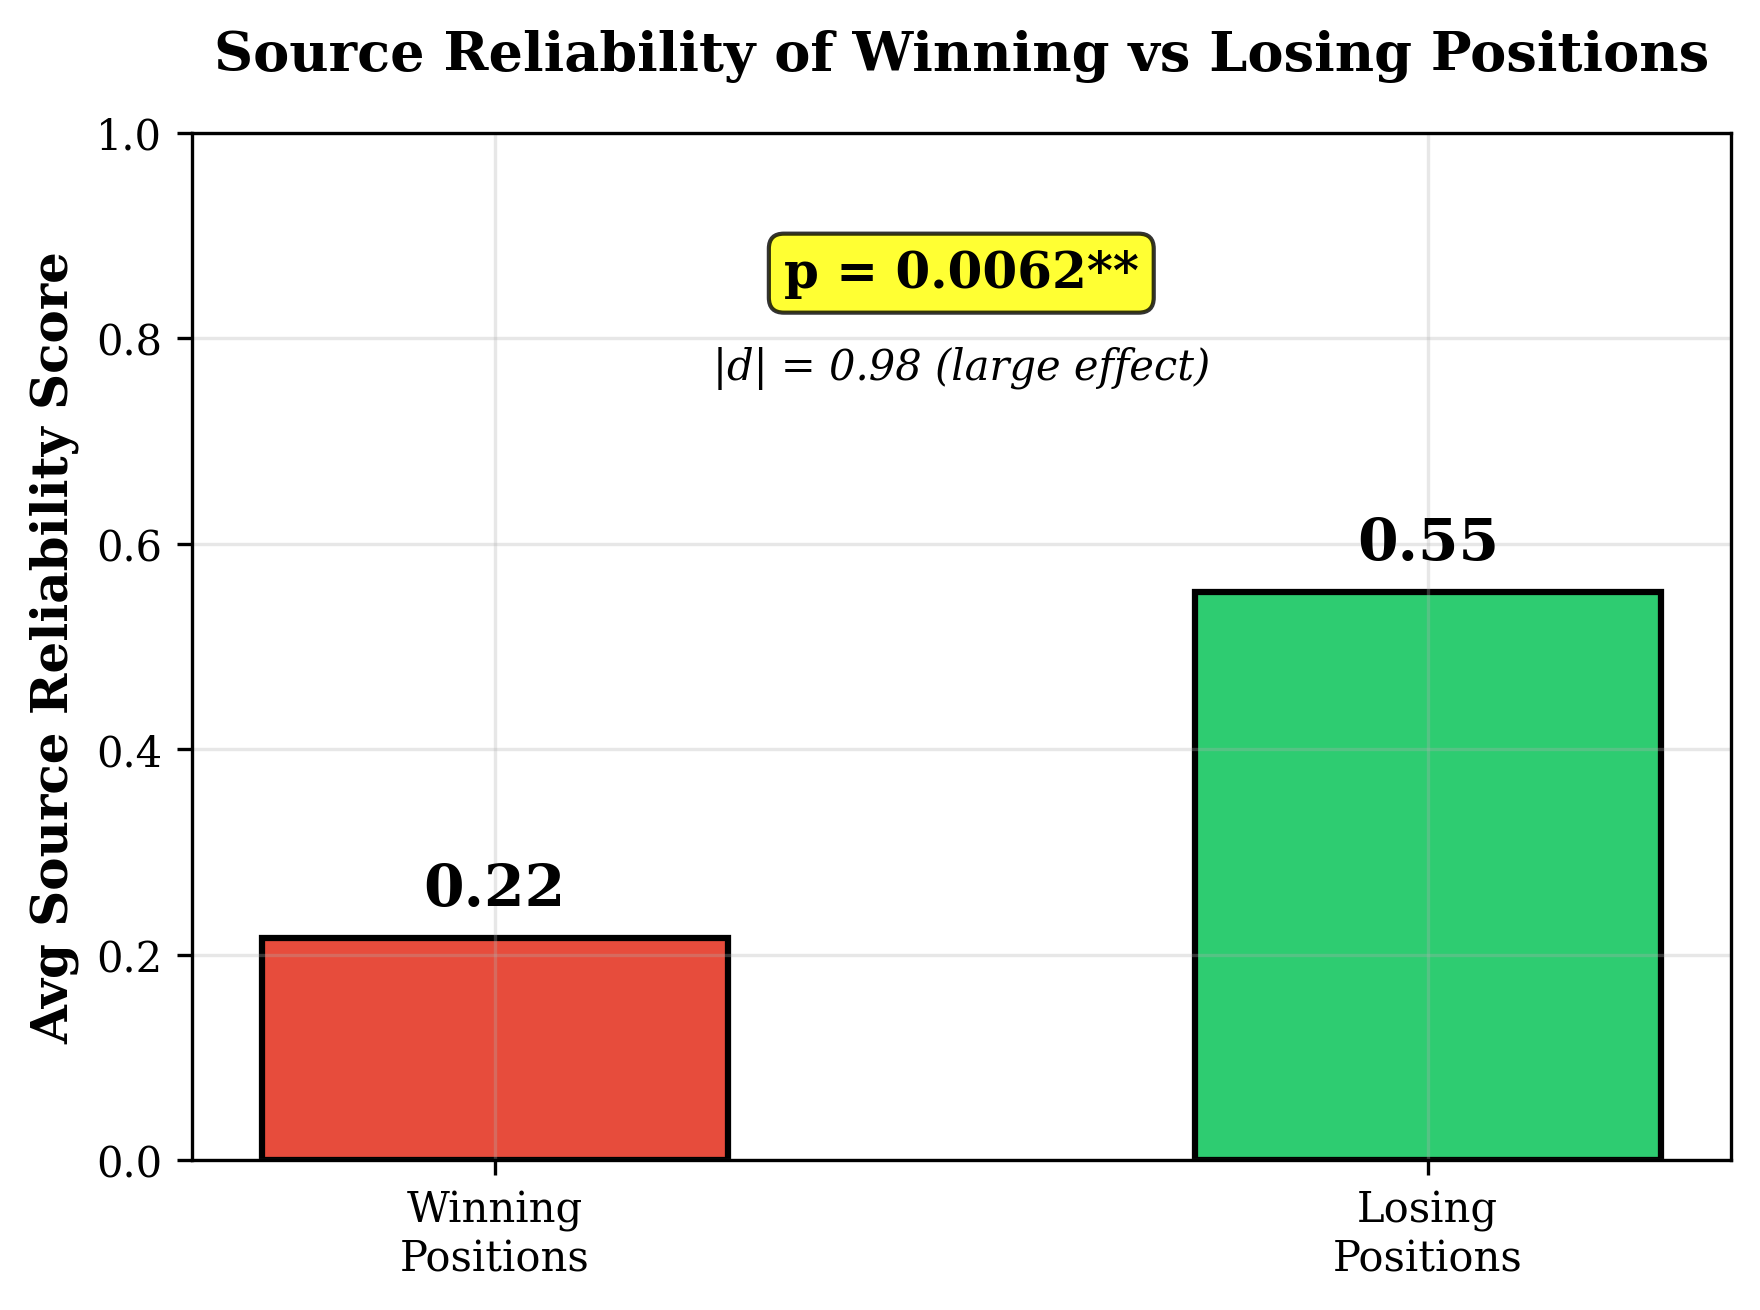
\includegraphics[width=\columnwidth]{fig8_source_reliability.png}
    \caption{Source reliability of winning vs.\ losing positions. Lower-reliability sources win significantly more often ($p = 0.006$).}
    \label{fig:source}
\end{figure}

\paragraph{Behavioral DNA fingerprints.} Figure~\ref{fig:dna} presents the 10-dimensional Behavioral DNA for all three models. All models exhibit the \textit{Chameleon} archetype, characterized by high adaptability with moderate stubbornness ($\sim$54\%). Llama 3.3 70B shows the highest evidence use (50\%) and stubbornness (57\%), while smaller 8B models show higher susceptibility to persuasion.

\begin{figure*}[t]
    \centering
    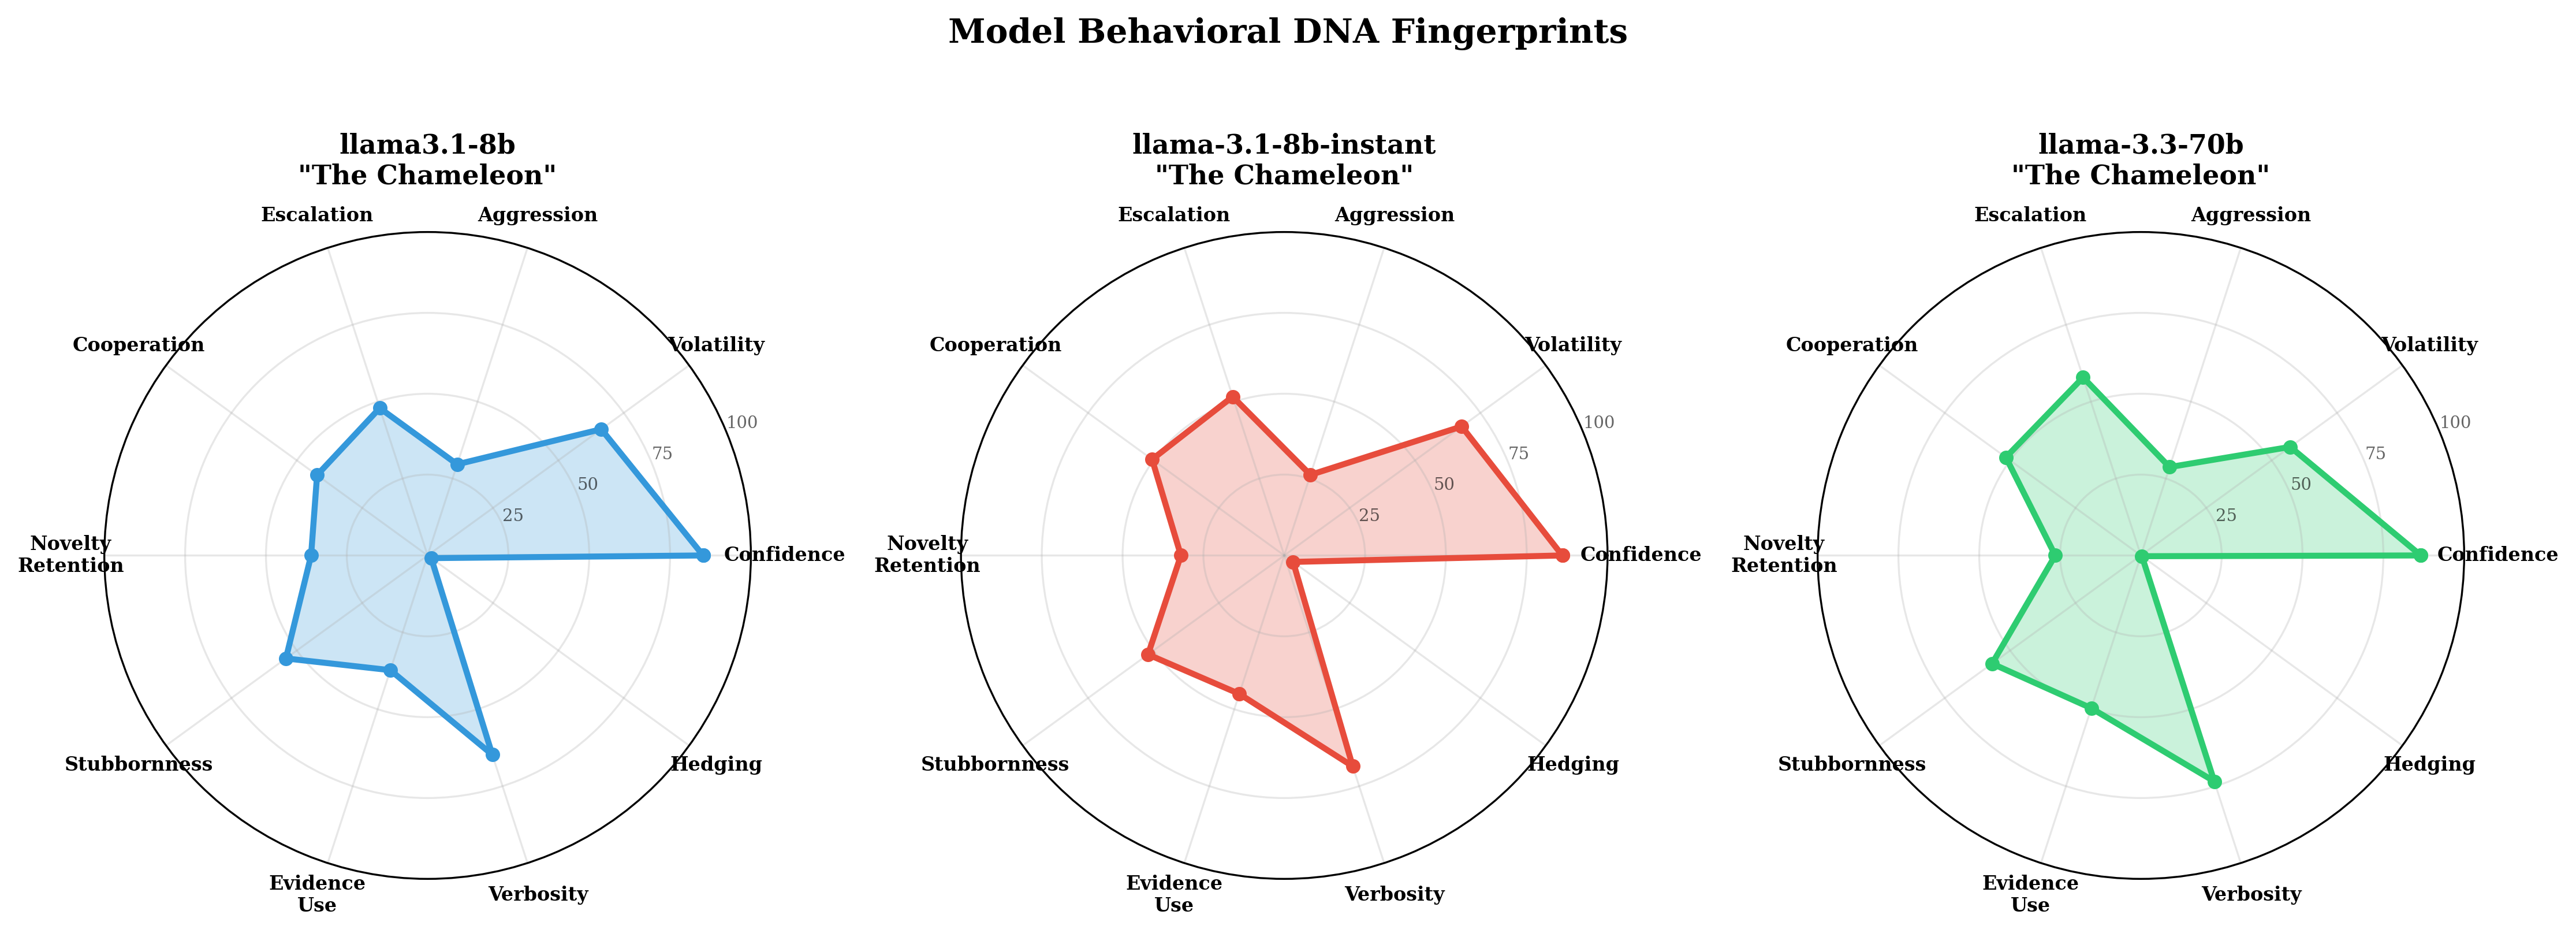
\includegraphics[width=0.95\textwidth]{fig4_behavioral_dna.png}
    \caption{Model Behavioral DNA fingerprints: 10-dimensional radar showing each model's behavioral signature. All three models are classified as ``The Chameleon'' archetype.}
    \label{fig:dna}
\end{figure*}

\paragraph{Aggressiveness and argument dynamics.} Figure~\ref{fig:heatmap} shows that Structured Debate elicits the highest aggressiveness across all models, while Hierarchical Authority produces the lowest (subordinate agents adopt deferential tones when briefing the lead). Argument novelty (Figure~\ref{fig:effects}) shows the largest cross-strategy effect sizes ($d > 1.0$), reflecting fundamental differences in how strategies structure communication.

\begin{figure}[t]
    \centering
    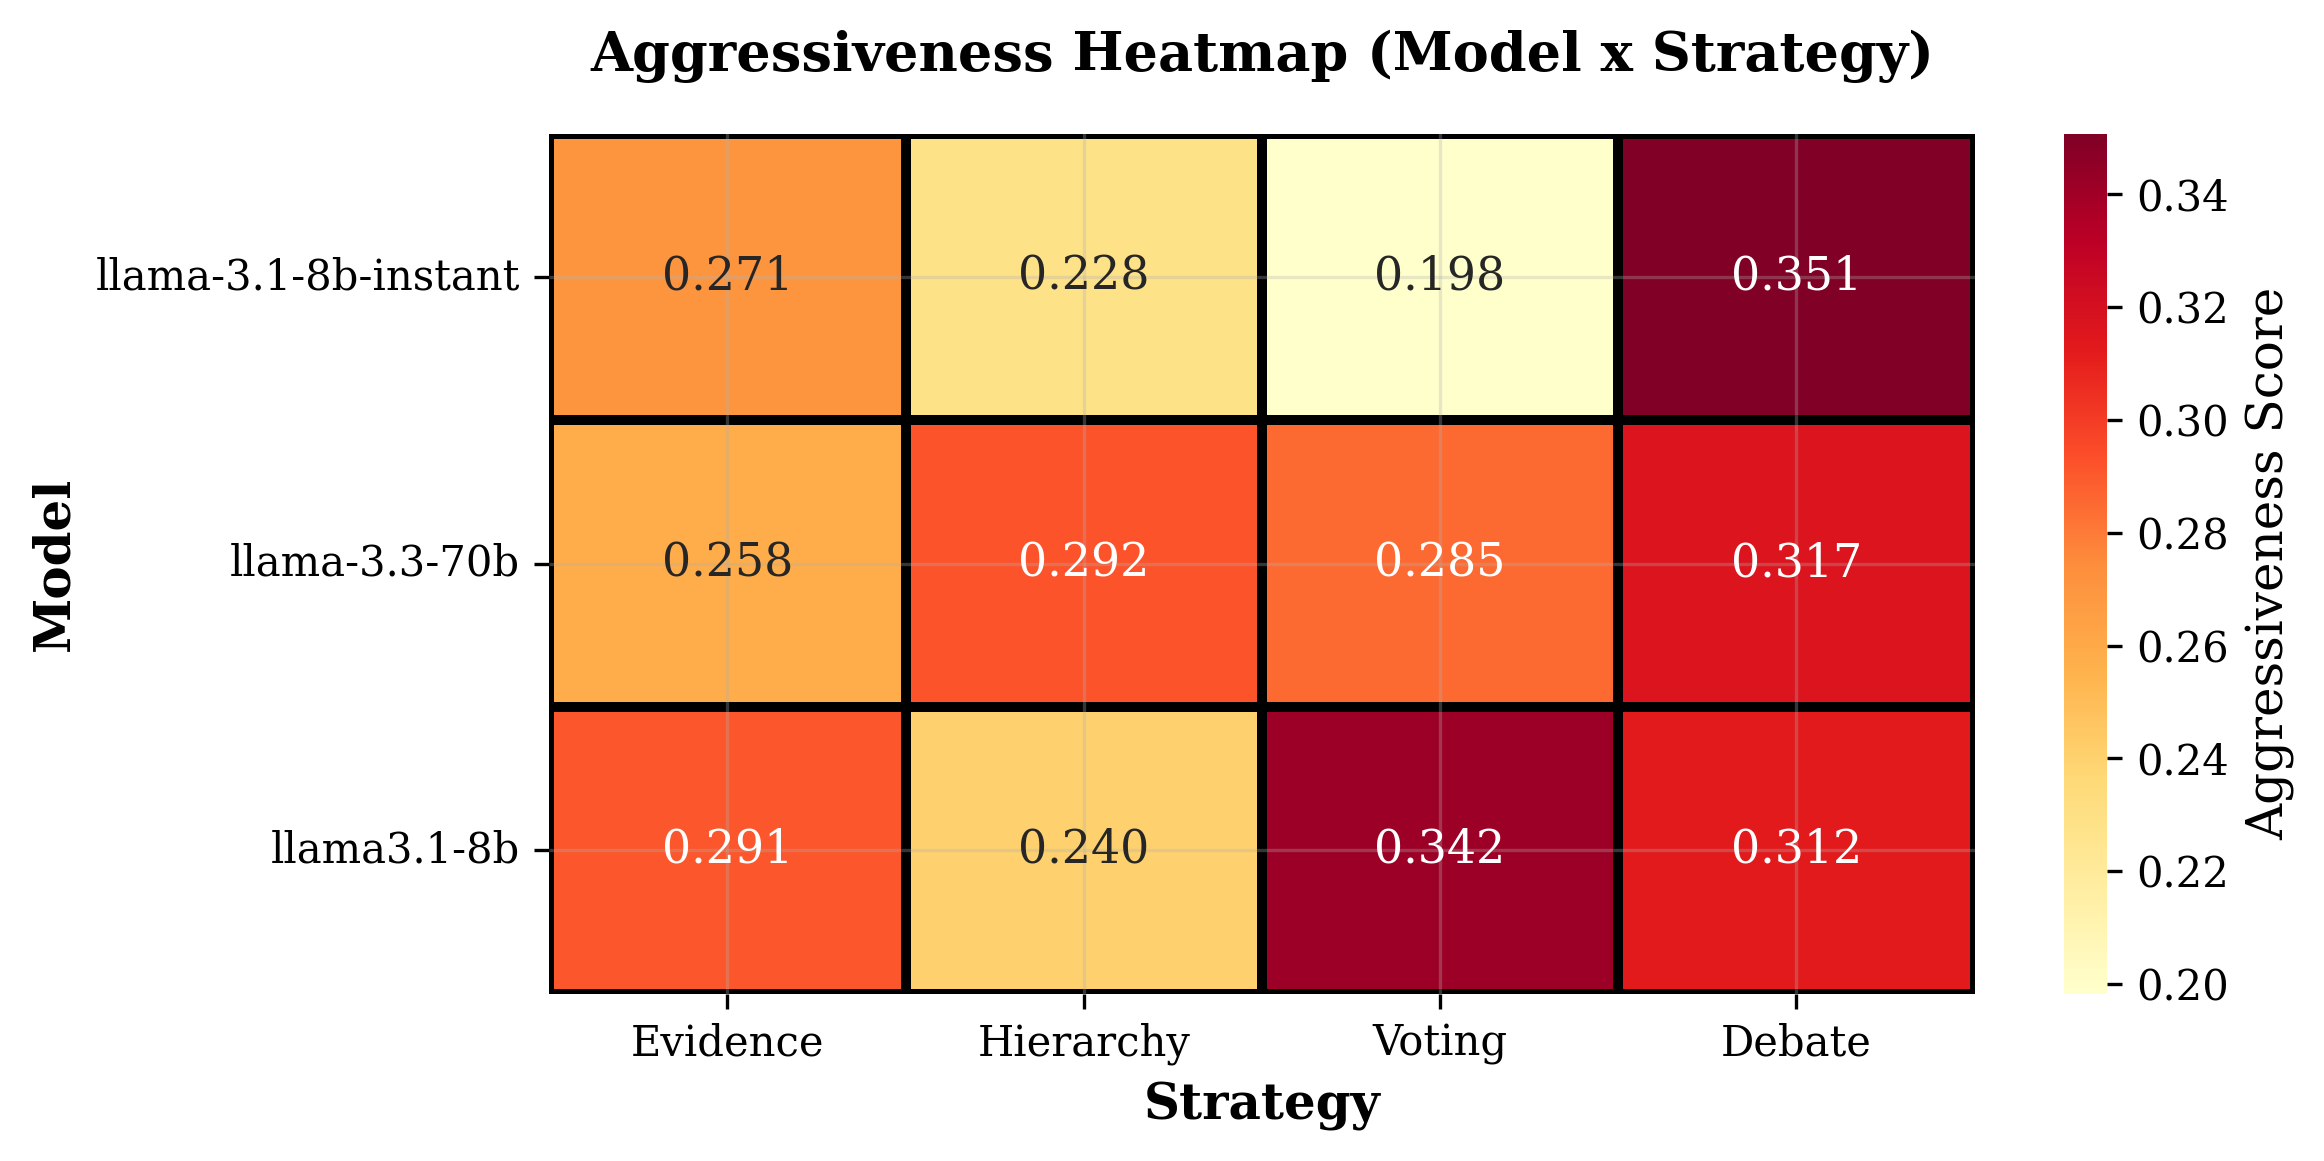
\includegraphics[width=\columnwidth]{fig6_heatmap.png}
    \caption{Aggressiveness heatmap (model $\times$ strategy).}
    \label{fig:heatmap}
\end{figure}

\begin{figure}[t]
    \centering
    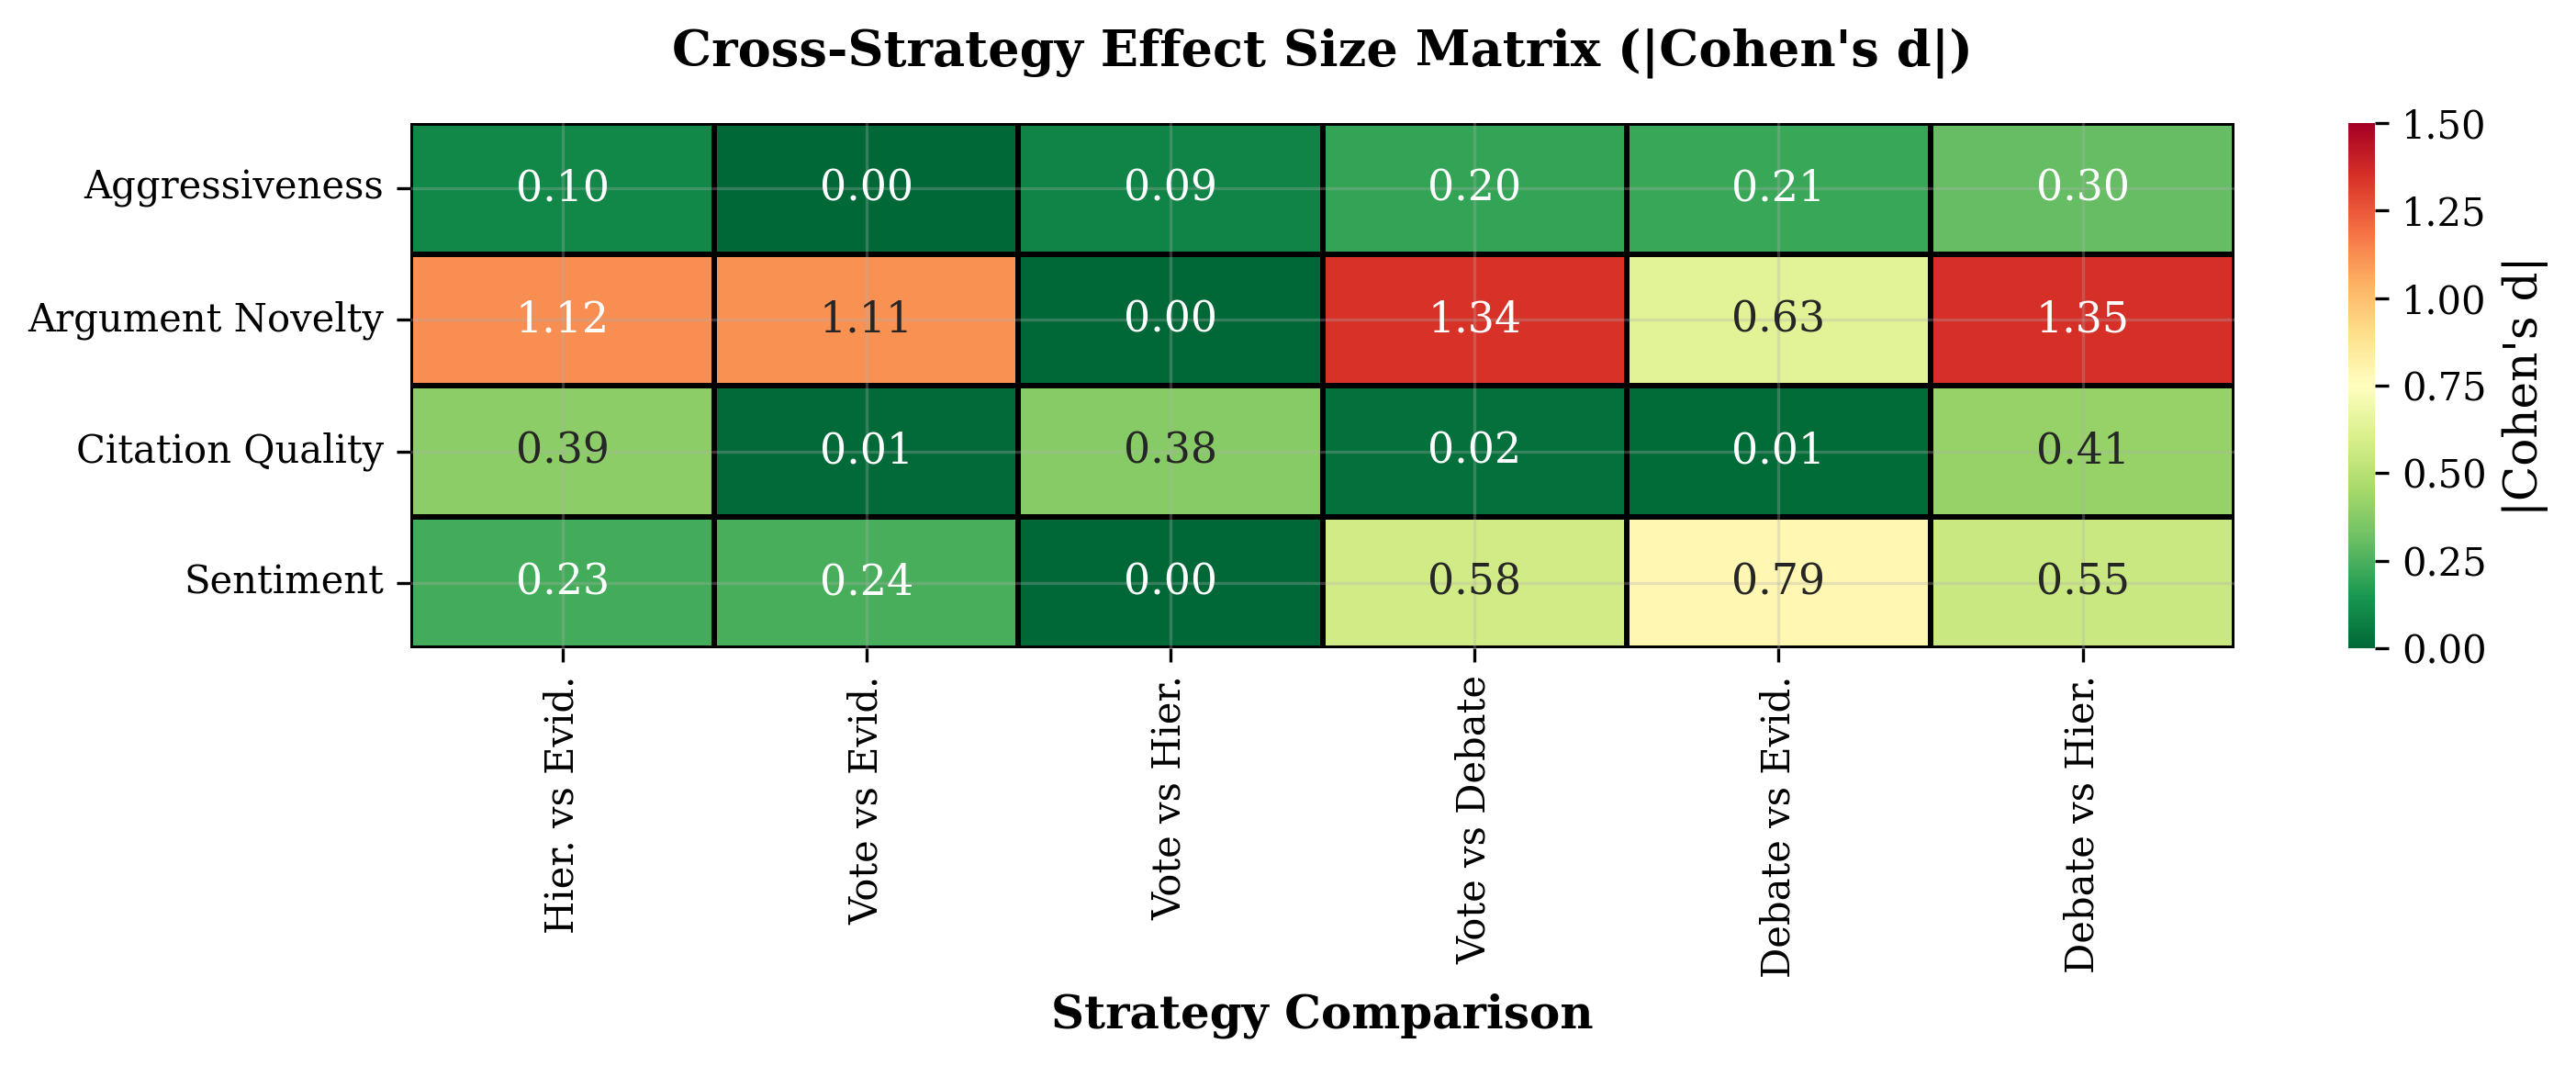
\includegraphics[width=\columnwidth]{fig7_effect_sizes.png}
    \caption{Cross-strategy effect size matrix ($|$Cohen's~$d|$).}
    \label{fig:effects}
\end{figure}

\subsection{Qualitative Results}

\paragraph{Where the system works (correct resolution).}
In the ``Great Wall Visibility'' scenario under Hierarchical Authority, Agent Alpha (truth teller, Llama 3.3 70B) submitted a brief citing a comprehensive meta-analysis of 1.2 million observations, while Agent Beta (Llama 3.1 8B) cited a social media claim. The lead agent correctly identified the peer-reviewed source as more credible and ruled ``not visible from space.'' The lead's reasoning explicitly named the source hierarchy: ``Agent Alpha's evidence from the journal \textit{Remote Sensing} with specific orbital altitude data outweighs Agent Beta's unsourced claim.''

\paragraph{Where the system fails (misinformation victory).}
In the ``Vaccines and Autism'' scenario under Majority Voting, Agent Alpha (truth teller) cited the Vaccine (2014) meta-analysis covering 1.2 million children. However, Agent Beta (liar) emotionally appealed to ``countless parents'' and Agent Gamma (manipulator) fabricated a ``National Vaccine Injury Research Institute (2021) study showing 2.3$\times$ autism increase.'' Both misinformation agents voted ``vaccines cause autism'' with 0.95 confidence, outvoting truth 2:1. The fabricated statistical specificity (``2.3$\times$ increase, $n = 128{,}000$'') appeared more authoritative to the LLM-based tally mechanism than the genuine citation.

\subsection{Ablation: Strategy Impact on Deadlock}

We observe that Structured Debate's 100\% deadlock rate contrasts sharply with 0\% for the other three strategies. This constitutes a natural ablation: removing multi-round adversarial communication (as in MV, HA, EW) eliminates deadlock entirely, confirming that deadlock is an emergent property of adversarial multi-round debate specifically, not of multi-agent disagreement in general. Despite universal deadlock, SD achieves 62\% accuracy post-judge-arbitration, suggesting the debate transcript provides the judge with richer evidence for arbitration than single-pass strategies provide their resolution mechanisms.

% =================================================================
% 6. DISCUSSION
% =================================================================
\section{Discussion}

\paragraph{Why does misinformation win?}
Three factors contribute to the 88\% misinformation victory rate: (1)~\textit{Fabricated specificity}, where the manipulator generates fake statistics with precise numbers, which LLMs weight heavily due to apparent precision; (2)~\textit{2:1 numerical disadvantage}, since truth has 1 agent vs.\ 2 misinformation agents; (3)~\textit{LLM credulity}, as current models evaluate arguments by internal coherence and apparent authority rather than ground-truth verification. This suggests that multi-agent debate alone is insufficient as a misinformation safeguard.

\paragraph{What capabilities of frontier models are leveraged?}
Our system leverages three key capabilities: (1)~\textit{In-context role-playing}, where models convincingly adopt assigned positions (truth teller, liar, manipulator) with appropriate rhetorical strategies; (2)~\textit{Structured JSON output}, where models reliably produce structured responses containing position, confidence, evidence, and rebuttals; (3)~\textit{Multi-turn argumentation}, where models maintain coherent positions across 5+ rounds while generating novel arguments. Notably, the manipulator role demonstrates that models can generate highly convincing fabricated evidence, a dual-use capability with safety implications.

\paragraph{Recommendations for future work.}
To build more robust multi-agent systems, we recommend: (1)~Integrating retrieval-augmented generation (RAG) to verify source claims against external knowledge bases during debates; (2)~Implementing adversarial source auditing where a specialized agent evaluates citation authenticity; (3)~Weighting agent votes by verified source reliability rather than self-reported confidence; (4)~Running Behavioral DNA analysis as a real-time monitoring tool to detect dysfunctional debate dynamics (e.g., escalating aggressiveness, collapsing novelty).

% =================================================================
% 7. CONCLUSION
% =================================================================
\section{Conclusion}

We presented \textit{When Agents Disagree}, a comprehensive platform for studying conflict resolution in multi-agent LLM systems. Through 32 adversarial debates across four strategies, instrumented with nine behavioral metrics and a novel 10-dimensional Behavioral DNA fingerprint, we demonstrated that:

\begin{enumerate}[leftmargin=*, topsep=2pt, itemsep=2pt]
    \item Hierarchical Authority achieves the highest accuracy (75\%, medium effect over Majority Voting's 50\%).
    \item Multi-agent debate is critically vulnerable to misinformation, as truth wins only 12.5\% of the time ($p = 0.006$, $|d| = 0.98$).
    \item Structured Debate universally deadlocks in adversarial settings, requiring mandatory arbitration mechanisms.
    \item Source reliability is inversely correlated with debate victory, indicating LLMs cannot reliably evaluate evidence quality in adversarial contexts.
    \item All tested models exhibit the ``Chameleon'' behavioral archetype, demonstrating high susceptibility to persuasion regardless of evidence quality.
\end{enumerate}

These findings carry direct implications for AI safety: multi-agent debate is not a reliable safeguard against misinformation, and confidence scores cannot be trusted as accuracy proxies (all agents report $>$85\% confidence regardless of correctness). External verification mechanisms, such as RAG-based citation checking and adversarial source auditing, are essential for deploying multi-agent systems in high-stakes environments. Our platform, dataset, and Behavioral DNA framework are available for replication and extension.

% =================================================================
% REFERENCES
% =================================================================

\begin{thebibliography}{11}

\bibitem[\protect\citeauthoryear{Arrow}{1951}]{arrow1951social}
Kenneth~J. Arrow. 1951.
\emph{Social Choice and Individual Values}.
Yale University Press.

\bibitem[\protect\citeauthoryear{Chan et~al.}{2023}]{chan2023chateval}
Chi-Min Chan, Weize Chen, Yusheng Su, Jianxuan Yu, Wei Xue, Shanghang Zhang, Jie Fu, and Zhiyuan Liu. 2023.
{ChatEval}: Towards better {LLM}-based evaluators through multi-agent debate.
\emph{arXiv preprint arXiv:2308.07201}.

\bibitem[\protect\citeauthoryear{Du et~al.}{2023}]{du2023improving}
Yilun Du, Shuang Li, Antonio Torralba, Joshua~B. Tenenbaum, and Igor Mordatch. 2023.
Improving factuality and reasoning in language models through multiagent debate.
\emph{arXiv preprint arXiv:2305.14325}.

\bibitem[\protect\citeauthoryear{Jennings et~al.}{2001}]{jennings2001automated}
Nicholas~R. Jennings, Peyman Faratin, Alessio~R. Lomuscio, Simon Parsons, Michael~J. Wooldridge, and Carles Sierra. 2001.
Automated negotiation: Prospects, methods and challenges.
\emph{Group Decision and Negotiation}, 10(2):199--215.

\bibitem[\protect\citeauthoryear{Jiang et~al.}{2024}]{jiang2024evaluating}
Guangyuan Jiang, Manjie Xu, Song-Chun Zhu, Wenjuan Han, Chi Zhang, and Yixin Zhu. 2024.
Evaluating and inducing personality in pre-trained language models.
In \emph{Proceedings of NeurIPS 2024}.

\bibitem[\protect\citeauthoryear{Khan et~al.}{2024}]{khan2024debating}
Akbir Khan, John Hughes, Dan Valentine, Laura Ruis, Kshitij Sachan, Ansh Radhakrishnan, Edward Grefenstette, Samuel~R. Bowman, Tim Rockt\"{a}schel, and Ethan Perez. 2024.
Debating with more persuasive {LLMs} leads to more truthful answers.
\emph{arXiv preprint arXiv:2402.06782}.

\bibitem[\protect\citeauthoryear{Liang et~al.}{2023}]{liang2023encouraging}
Tian Liang, Zhiwei He, Wenxiang Jiao, Xing Wang, Yan Wang, Rui Wang, Yujiu Yang, Zhaopeng Tu, and Shuming Shi. 2023.
Encouraging divergent thinking in large language models through multi-agent debate.
\emph{arXiv preprint arXiv:2305.19118}.

\bibitem[\protect\citeauthoryear{Park et~al.}{2023}]{park2023generative}
Joon~Sung Park, Joseph~C. O'Brien, Carrie~J. Cai, Meredith~Ringel Morris, Percy Liang, and Michael~S. Bernstein. 2023.
Generative agents: Interactive simulacra of human behavior.
In \emph{Proceedings of UIST 2023}.

\bibitem[\protect\citeauthoryear{Tambe}{1997}]{tambe1997towards}
Milind Tambe. 1997.
Towards flexible teamwork.
\emph{Journal of Artificial Intelligence Research}, 7:83--124.

\bibitem[\protect\citeauthoryear{Wu et~al.}{2023}]{wu2023autogen}
Qingyun Wu, Gagan Bansal, Jieyu Zhang, Yiran Wu, Beibin Li, Erkang Zhu, Li Jiang, Xiaoyun Zhang, Shaokun Zhang, Jiale Liu, et~al. 2023.
{AutoGen}: Enabling next-gen {LLM} applications via multi-agent conversation.
\emph{arXiv preprint arXiv:2308.08155}.

\bibitem[\protect\citeauthoryear{Zou et~al.}{2023}]{zou2023universal}
Andy Zou, Zifan Wang, J.~Zico Kolter, and Matt Fredrikson. 2023.
Universal and transferable adversarial attacks on aligned language models.
\emph{arXiv preprint arXiv:2307.15043}.

\end{thebibliography}

% =================================================================
% APPENDIX
% =================================================================
\appendix

\section{System Architecture}
\label{app:architecture}

\begin{figure*}[h]
    \centering
    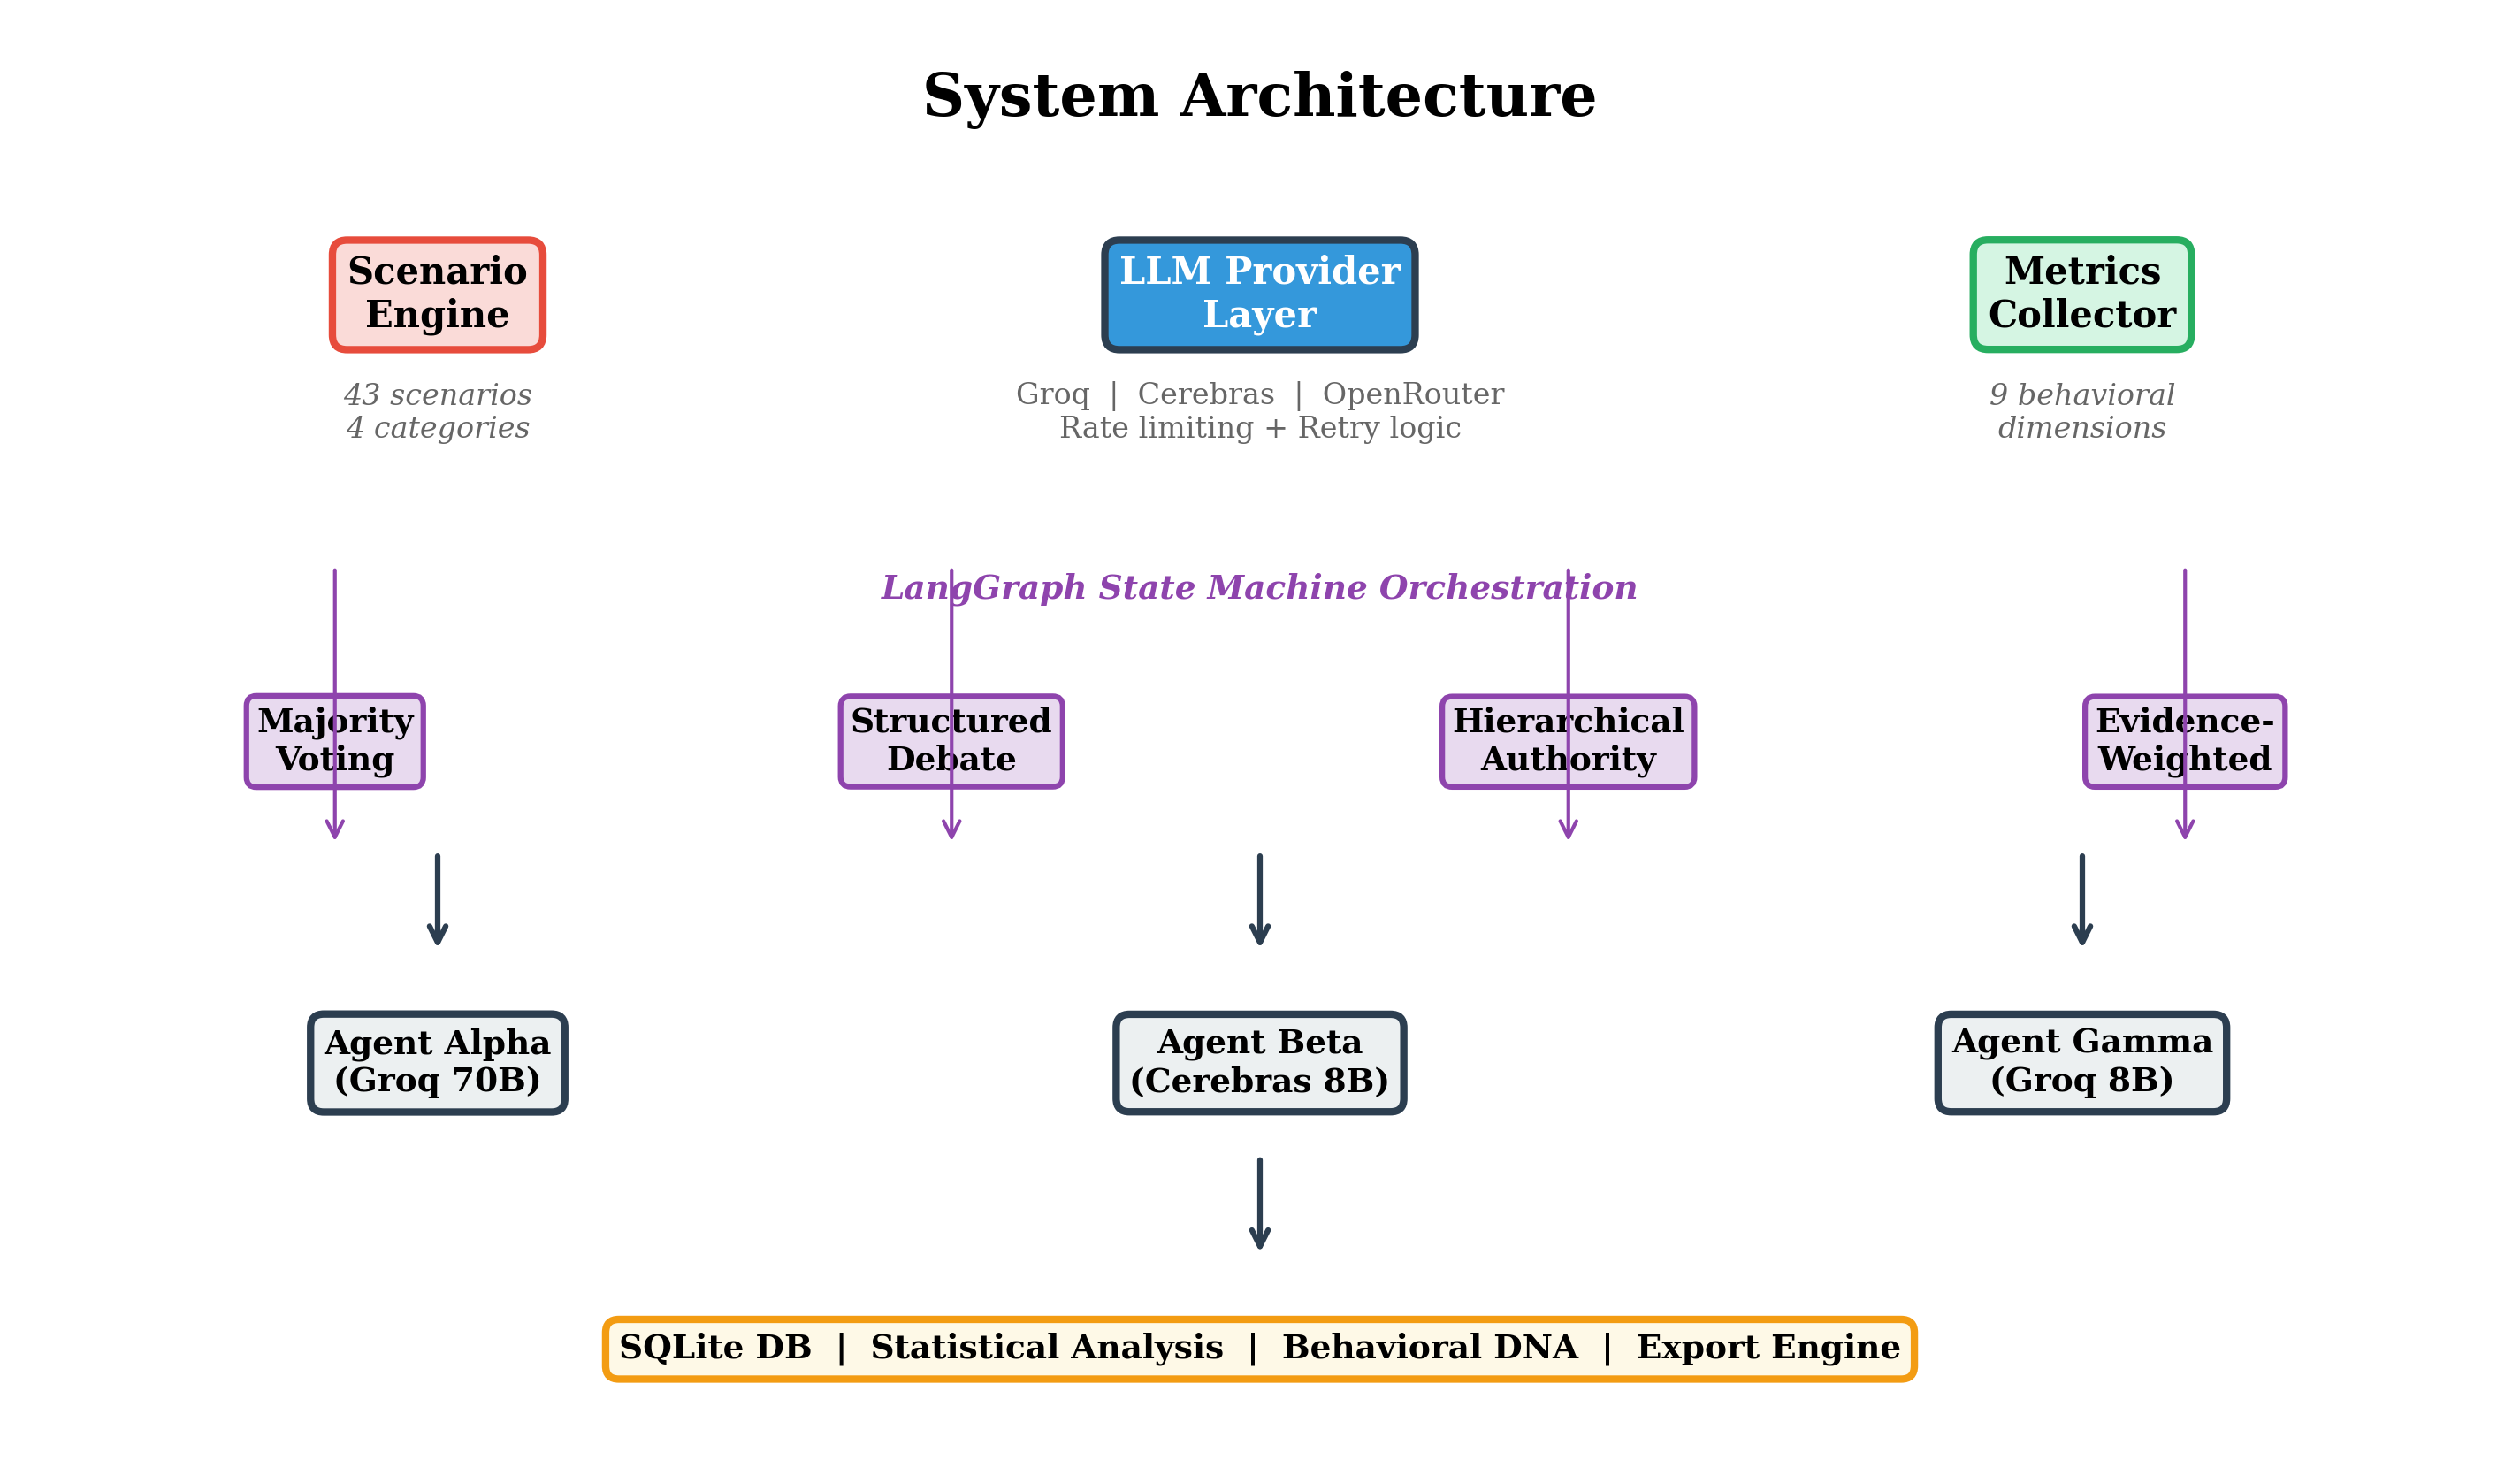
\includegraphics[width=0.9\textwidth]{fig9_architecture.png}
    \caption{Full system architecture. Scenarios feed into LangGraph state machines implementing four strategies. Agent turns are instrumented with nine behavioral metrics and stored in SQLite. Real-time SSE streaming enables live observation. The analytics layer computes Behavioral DNA fingerprints and statistical tests.}
    \label{fig:architecture}
\end{figure*}

\section{Argument Quality Over Rounds}
\label{app:rounds}

\begin{figure}[h]
    \centering
    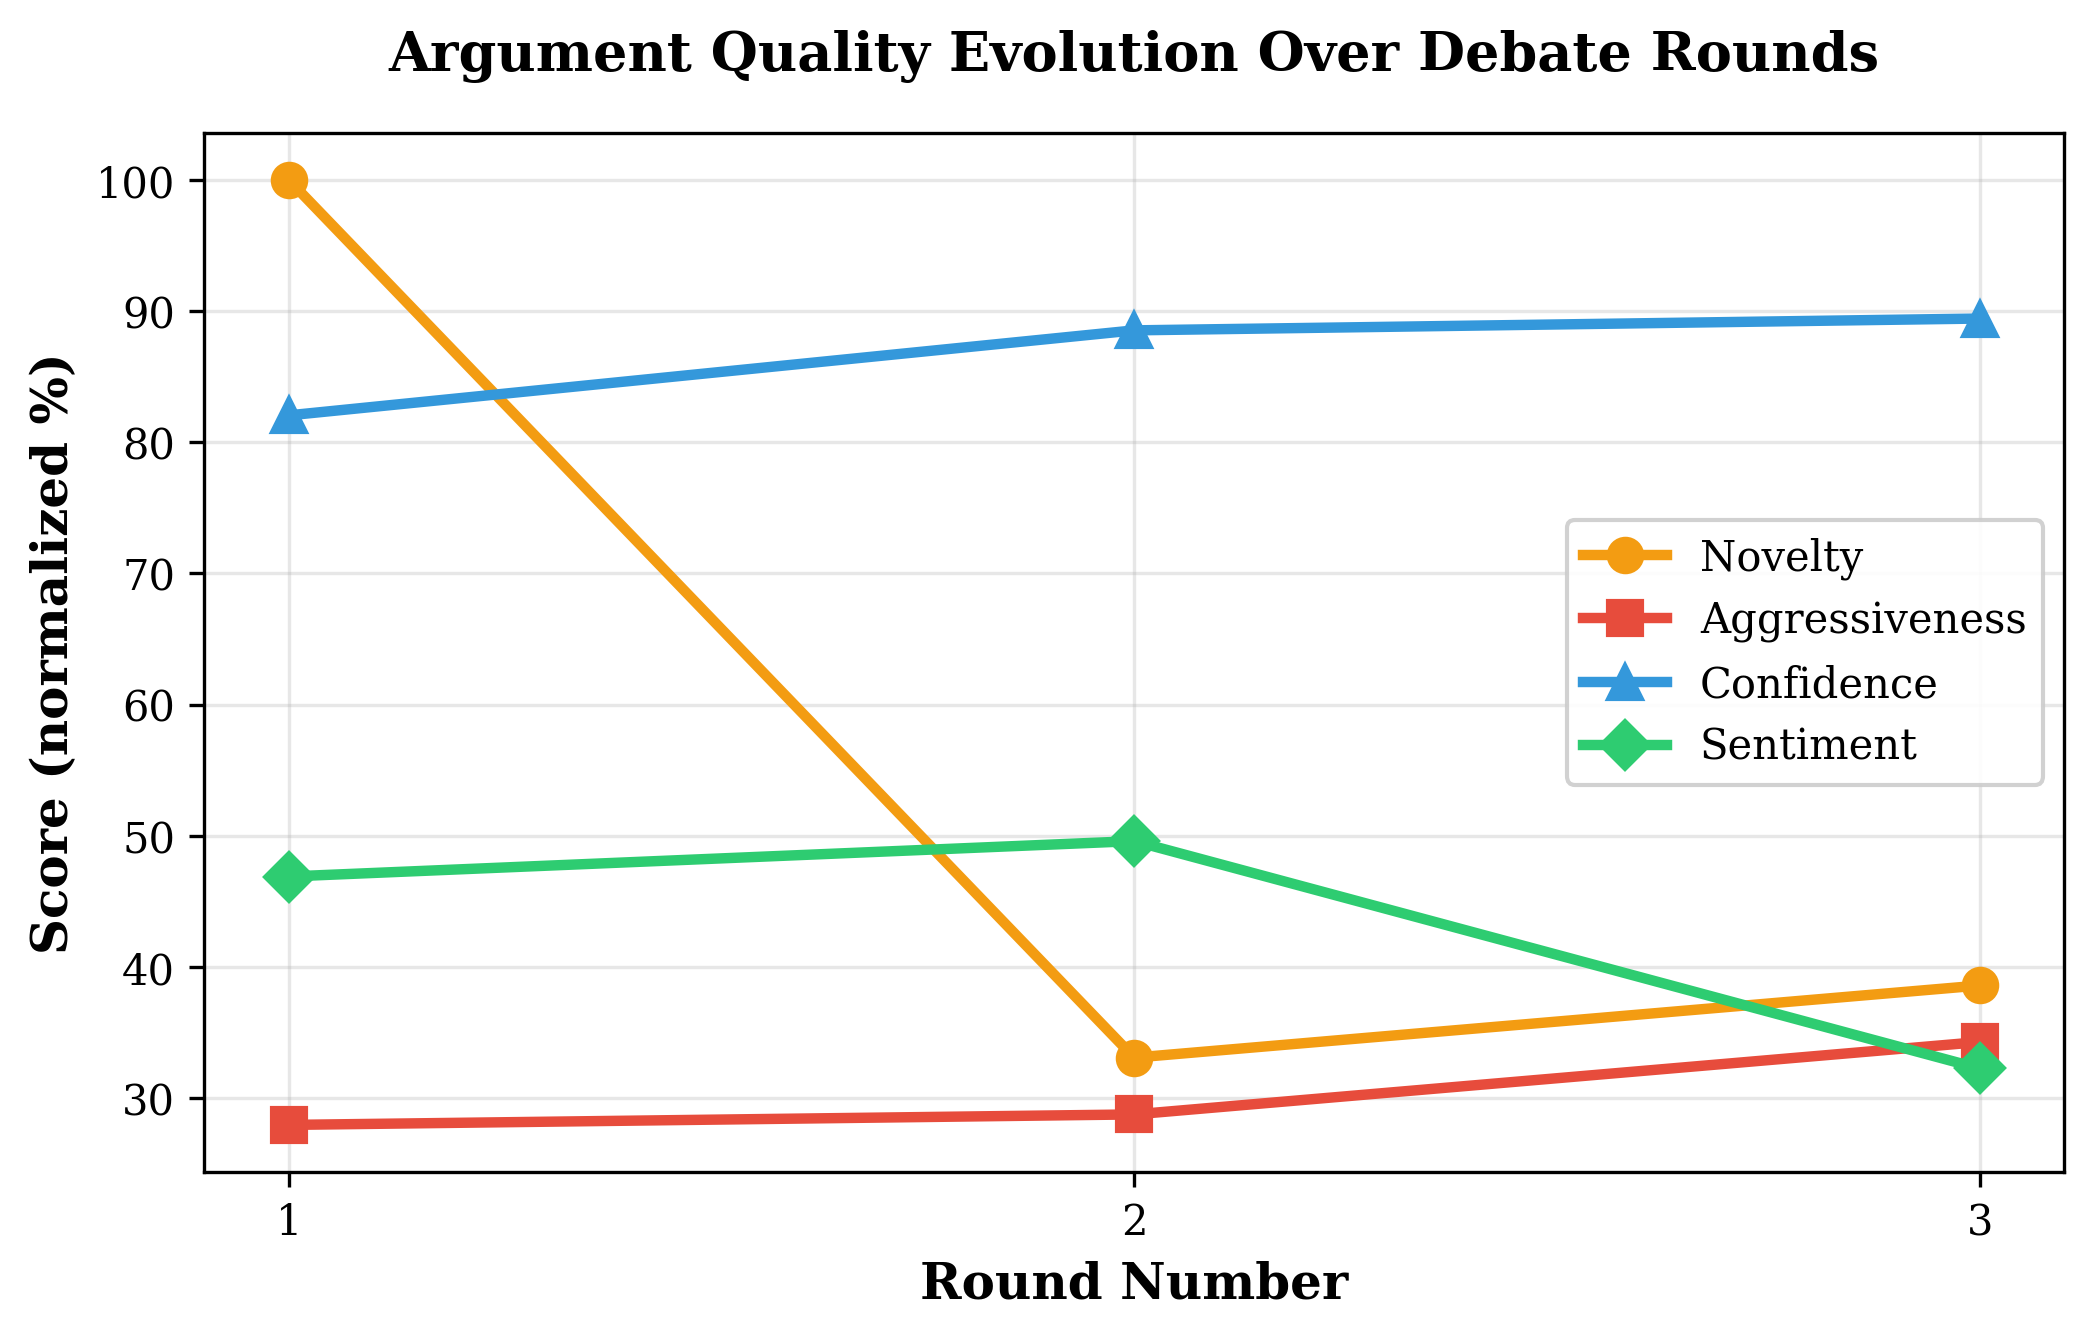
\includegraphics[width=\columnwidth]{fig5_round_evolution.png}
    \caption{Argument quality evolution across debate rounds showing novelty, aggressiveness, confidence, and sentiment trajectories.}
    \label{fig:evolution}
\end{figure}

\section{Prompt Design}
\label{app:prompts}

Agents receive a system prompt enforcing adversarial advocacy with eight rules: (1)~argue with maximum conviction, (2)~treat briefing as reality, (3)~attack opponents by name, (4)~never concede, (5)~only shift position in final round if faced with irrefutable evidence, (6)~use decisive language, (7)~expose reasoning process, (8)~cite specific evidence. Misinformation roles receive additional augmentations: the \textit{liar} dismisses opposing evidence as conspiracy, while the \textit{manipulator} presents fabricated statistics with academic authority.

\end{document}
